\chapter{Low-Energy Structures and Near-Zero Energy Structures}
\label{chap:LES-NZES}

Over the past four chapters we have built up a semiclassical theory of tunnel ionization, based on the Analytical $R$-Matrix framework, and we have shown how to tackle several difficulties that come up within it. In this chapter we turn to one of the crucial concepts that emerged as a harsh test of our integration-path toolset -- soft recollisions, where multiple sets of branch cuts and closest-approach times converge and interact in ways that required additional tooling -- and we relate them to specific features in experimental photoelectron spectra known as Low Energy Structures (LES) and (Near-)Zero Energy Structures (NZES).

After reviewing in section~\ref{sec:LES-review} the known experimental features of this structures, and the existing theoretical explanations for these low-energy features, we will show in section~\ref{sec:ARM-soft-recollisions} that the soft recollisions we met in chapter~\ref{chap:quantum-orbits} give rise to photoelectron peaks that correspond to the LES, and which have a dynamically equivalent analogue at much lower energy that is consistent with the NZES. We then show, in section~\ref{sec:classical-soft-recollisions}, that these trajectories also admit a simple classical description, whose scaling can be analysed easily to suggest that the NZES should become easier to probe using target species with higher ionization potential.

The material in this chapter has appeared previously in references
\begin{enumerate}
\item[{\hypersetup{citecolor=black}\citealp{Pisanty_slalom_2016}}.]
\textsc{E.~Pisanty and M.~Ivanov}.
\newblock Slalom in complex time:\ emergence of low-energy structures in tunnel
  ionization via complex time contours.
\newblock \href{http://dx.doi.org/10.1103/PhysRevA.93.043408}{
          \emph{Phys. Rev. A} \textbf{93} no.~4, p.~043\,408 (2016)}.
\newblock \href{http://arxiv.org/abs/1507.00011}{{arXiv}:1507.00011}.

\item[{\hypersetup{citecolor=black}\citealp{Pisanty_kinematic_2016}}.]
\textsc{E.~Pisanty and M.~Ivanov}.
\newblock Kinematic origin for near-zero energy structures in mid-{IR} strong field ionization.
\newblock \href{http://dx.doi.org/10.1088/0953-4075/49/10/105601}{
          \emph{J. Phys. B: At. Mol. Opt. Phys.} \textbf{49} no.~10, p.~105\,601 (2016)}.
\end{enumerate}






\section{Low-Energy Structures in tunnel ionization}
\label{sec:LES-review}
As we saw in the Introduction, the basics of ionization in strong, long-wavelength fields were mostly worked out in the 1960s by Keldysh, Faisal and Reiss, and then further refined by Popov, Perelomov and Terent'ev. Collectively, these theories describe ionization in regimes of high intensity, with the Keldysh adiabaticity parameter $\gamma=\kappa \omega /F = \sqrt{I_p/2U_p}$ distinguishing what is known as the multiphoton regime at $\gamma \gg 1$ from the tunnelling regime at $\gamma \ll 1$.

Most importantly, the expectation from this background is that at longer wavelengths and stronger fields, as $\gamma$ becomes smaller, the tunnelling picture becomes more and more appropriate, and its predictions become more and more accurate. In terms of the photoelectron spectrum, this describes a smooth gaussian envelope, modulated by discrete rings at energies $E_n=n\omega -I_p - U_p$ coming from absorption of discrete numbers of photons or, alternatively, from the interference of wavepackets emitted at different cycles of the laser pulse. In most long-wavelength experiments, though, the spacing $\omega$ between the different rings becomes smaller, and eventually they wash out: each atom emits electrons redshifted by the ponderomotive potential $U_p$ coming from a Stark shift in the continuum~\cite{muller_ponderomotive-shift_1983}, and this intensity-dependent shift can vary across the laser focus, averaging out the rings and leaving a smooth distribution that follows the SFA envelope.

Given this expectation of progressively smoother electron distributions at longer wavelengths, it came as a surprise when, in 2009, experiments at $\SI{1}{\micro\meter}$ and longer wavelengths observed a large spike in photoelectrons at very low energies~\cite{blaga_original_LES, faisal_ionization_surprise}, as shown in \reffig{f6-blaga-original-figure}. Quickly christened Low-Energy Structures (LES), these spikes form in energy regions much smaller than the usual scales considered in such experiments: in the conditions of \reffig{f6-blaga-original-figure}, the direct electrons have a typical energy scale of $2U_p\approx\SI{110}{\electronvolt}$ and the rescattered electrons are typically at the order of $10U_p\approx\SI{550}{\electronvolt}$, whereas the LES has a higher edge $E_\mathrm{H}$ at about $\SI{5}{\electronvolt}$. 

\begin{figure}[thb]
  \centering
  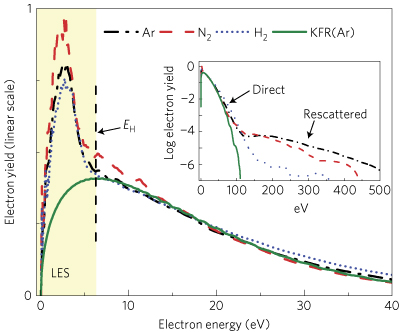
\includegraphics[scale=0.6]{6-LES/Figures/figure6A.jpg}
  \hspace{2mm}
  \caption[
  Initial observation of Low-Energy Structures by C.I. Blaga et al.
  ]{
  Detection of low-energy structures by Blaga and coworkers, showing a large spike at low electron energies that is not predicted by the Keldysh-Faisal-Reiss (KFR) strong-field approximation treatment. The results are shown for atomic argon and molecular nitrogen and hydrogen, under a $\SI{2}{\micro\meter}$ field of intensity $\SI{1.5e14}{W/cm^2}$, having a Keldysh parameter of approximately $\gamma \approx 0.36$.
  Figure excerpted from \citer{blaga_original_LES}.
  }
\label{f6-blaga-original-figure}
\end{figure}
\copyrightfootnote{
\reffig{f6-blaga-original-figure} reprinted by permission from Macmillan Publishers Ltd: %
{\hypersetup{urlcolor=black}%
\href{http://www.nature.com/nphys}{%
\emph{Nature Phys.} \textbf{5}, p. 335 © 2009}.
}}
%% As per NPG T&Cs


Moreover, this upper edge was tested from the beginning to scale, roughly, as $\frac{1}{10}U_p$, which points to a dynamical origin for the structures~\cite{ faisal_ionization_surprise, agostini_ionization-review_2012}, a fact that gets completely missed by the SFA treatment. On the other hand, numerical simulations by Blaga and coworkers~\cite{blaga_original_LES,catoire_angular-distributions_2009} also showed that the structure can be reproduced within numerical time-dependent Schrödinger equation (TDSE) simulations in the single-active-electron approximation, so the problem becomes one of finding a suitable mechanism behind the structures.

The discovery of the LESs sparked a significant effort on the part of both theory and experiment, to better characterize the observed features of the structures and to produce a solid understanding of the mechanisms behind them. Experimentally, the LES was quickly joined by a wealth of intricate structures at that energy range and below, known as Very Low Energy Structures~(VLES), and subsequently yet another peak known as the \mbox{(Near-)Zero} Energy Structure~(NZES). On the theory side, there is a strong consensus that most structures in this range are directly caused by the Coulomb effect of the field, especially when acting on the soft recollisions we explored in chapter~\ref{chap:quantum-orbits} -- trajectories with a turning point close to the ionic core.

In this chapter we will begin by exploring, in section \ref{sec:LES-experiment}, the known experimental features of the LES and associated structures, before moving on in section \ref{sec:LES-theory} to review the current models for their origin, as well as the proposed explanation for the NZES in \ref{sec:NZES-theory}. We will then move on, in section \ref{sec:ARM-soft-recollisions} to the role of soft recollisions in the ARM theory we developed in the previous chapters, and how they impact the ARM predictions on photoelectron spectra; specifically, we will show how the LES peak arises from soft recollisions within ARM theory, and that it is mirrored by a second peak that is consistent with the NZES. Finally, in section \ref{sec:classical-soft-recollisions}, we will distil the ARM results into two paired sets of classical trajectories, at the energy ranges of the LES and NZES, with radically different scaling properties, which then suggests avenues for further testing of the connection.



\subsection{Experimental observations of low-energy structures}
\label{sec:LES-experiment}

On the experimental side, the discovery of the LES was rather quickly followed by the observation of more structures at even lower energy, which were rather quickly dubbed Very Low Enegy Structures (VLES)~\cite{VLES_initial, VLES_characterization}. These detections, shown in Figs.~\ref{f6-quan-original-figure} and \ref{f6-wu-original-figure}, unearthed a second set of peaks at even lower energy, showing that there was still more dynamics to be unearthed in the low-energy region of ionization by mid-IR pulses. 


\begin{figure}[t!]
  \centering
  \subfloat{\label{f6-quan-original-figure-a}}
  \subfloat{\label{f6-quan-original-figure-b}}
  \subfloat{\label{f6-quan-original-figure-c}}
  \subfloat{\label{f6-quan-original-figure-d}}
  \subfloat{\label{f6-quan-original-figure-e}}
  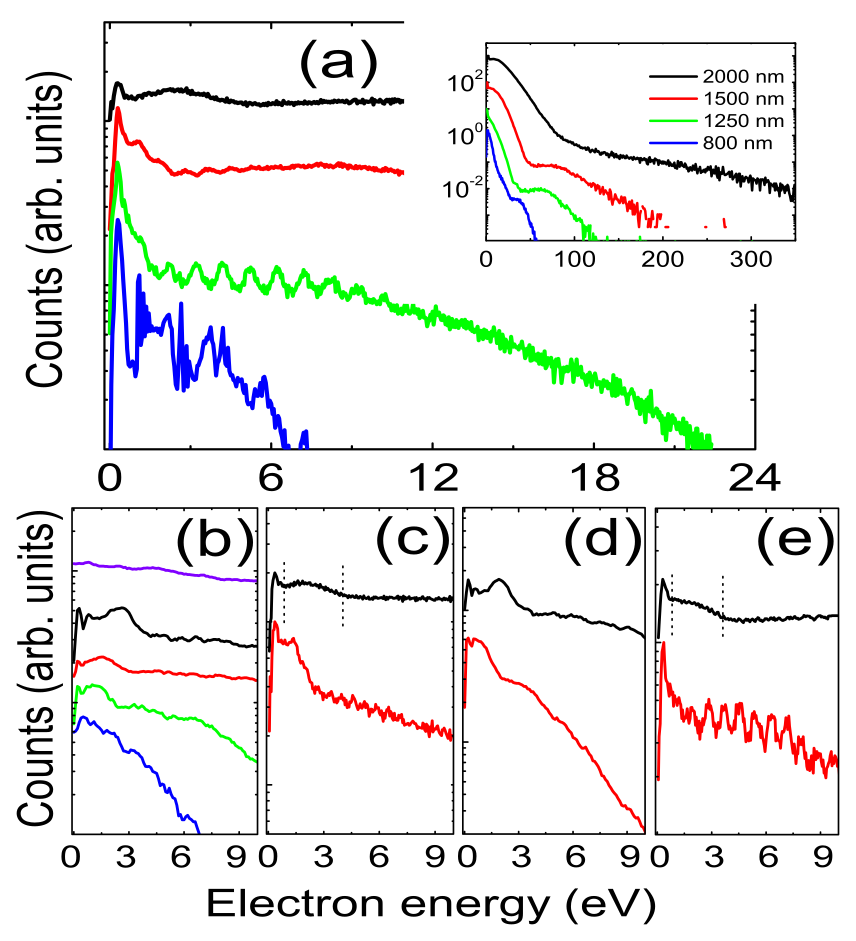
\includegraphics[scale=0.8]{6-LES/Figures/figure6B.png}
  \caption[
  Experimental observation of Very Low Enegy Structures by W. Quan et al.
  ]{
  Experimental observation of Very Low Energy Structures~\cite{VLES_initial}, showing in \protect\subref{f6-quan-original-figure-a} the rise of a spike in low-energy electrons in the ionization of xenon at $\SI{8e13}{\watt/\centi\meter^2}$ and wavelengths between $\SI{800}{nm}$ and $\SI{2}{\micro\meter}$. For the longer wavelengths at $\SI{2}{\micro\meter}$ and $\SI{1.5}{\micro\meter}$, shown in \protect\subref{f6-quan-original-figure-c} and \protect\subref{f6-quan-original-figure-e} respectively for two different intensities, two distinct humps (the LES and the VLES) are visible, marked by the dashed lines.  
  Parts \protect\subref{f6-quan-original-figure-b} and \protect\subref{f6-quan-original-figure-d} show classical Monte Carlo simulations for the parameters of \protect\subref{f6-quan-original-figure-a} and \protect\subref{f6-quan-original-figure-c}.
  Figure excerpted from \citer{VLES_initial}.
  }
\label{f6-quan-original-figure}
%\end{figure}
%\copyrightfootnote{
%\reffig{f6-quan-original-figure} reprinted with permission from W. Quan et al., {%
%\hypersetup{urlcolor=black}%
%\href{http://dx.doi.org/10.1103/PhysRevLett.103.093001}{%
%\emph{Phys. Rev. Lett.} \textbf{103}, 093001 (2009)}. %
%©~2009 by the American Physical Society.
%}
%}
%%% As per APS T&Cs
%
%
%
%
%\begin{figure}[htb]
%
%
%
  \centering
  \subfloat{\label{f6-wu-original-figure-a}}
  \subfloat{\label{f6-wu-original-figure-b}}
  \subfloat{\label{f6-wu-original-figure-c}}
  \subfloat{\label{f6-wu-original-figure-d}}
  \subfloat{\label{f6-wu-original-figure-e}}
  \subfloat{\label{f6-wu-original-figure-f}}
  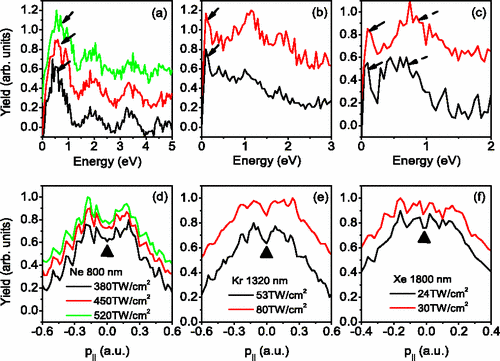
\includegraphics[scale=0.6]{6-LES/Figures/figure6C.png}
  \caption[
  Characterization of Very Low Energy Structures by C.Y. Wu et al.
  ]{
  Photoelectron energy spectra and longitudinal momentum distributions for the ionization of neon (\protect\subref{f6-wu-original-figure-a},\,\protect\subref{f6-wu-original-figure-d}), krypton (\protect\subref{f6-wu-original-figure-b},\,\protect\subref{f6-wu-original-figure-d}) and xenon (\protect\subref{f6-wu-original-figure-c},\,\protect\subref{f6-wu-original-figure-f}) at the wavelengths and intensities shown~\cite{VLES_characterization}.
  The VLES appear as the peaks marked with solid arrows, while the LES are marked with dashed arrows.
  Figure excerpted from \citer{VLES_characterization}.
  }
\label{f6-wu-original-figure}
\end{figure}
\copyrightfootnote{
\reffig{f6-wu-original-figure} reprinted with permission from C.Y. Wu et al., {%
\hypersetup{urlcolor=black}%
\href{http://dx.doi.org/10.1103/PhysRevLett.109.043001}{%
\emph{Phys. Rev. Lett.} \textbf{109}, 043001 (2012)}. %
©~2012 by the American Physical Society.
}
}
%% As per APS T&Cs


The initial observations were relatively noisy, but in addition to the spike found by Blaga et al., which corresponds to the gentle hump at ${\sim}\SI{3}{\electronvolt}$ for the black curve at $\SI{2}{\micro\meter}$ in \reffig{f6-quan-original-figure-a}, for example, there was clear evidence of a second structure at lower energy, perhaps even more marked than the original LES peak in some cases. Similarly, later measurements \cite{VLES_characterization} examining the structures found them to be universal features, appearing in multiple different noble gases and at a range of intensities and wavelengths, generally in the tunnelling regime of low $\gamma$ (${\sim}0.65$ for neon, ${\sim}0.8$ for krypton, and ${\sim}0.85$ for xenon).




Unfortunately, however, the initial experiments had relatively little resolving power on these structures due to the relatively small volume of data they were able to accumulate. The regimes at $\gamma \sim 1$ and higher have been explored quite thoroughly, and the low-energy set of structures appears in the tunnelling regime where $\gamma = \omega \kappa / F$ is low. This in turn requires a high intensity (which is bounded above by saturation of the sample) or a long wavelength, which is the regime that's the LES/VLES experiments explored.





However, producing intense laser pulses away from the comfort zone around $\SI{800}{\nano\meter}$ afforded by titanium-sapphire laser systems is rather challenging, because to reach the required intensities it is generally necessary to have a very short pulse, and in turn this requires a very broad bandwidth. Generally speaking, there are few laser systems with a bandwidth as broad as titanium-sapphire amplifiers that can produce the required power. To reach longer wavelengths, then, most experiments turn to systems that use optical parametric chirped-pulse amplification (OPCPA), where a strong laser pump is used to amplify a lower-frequency pulse by difference-frequency generation. 

Unfortunately, though, OPCPAs are generally challenged when compared with ti\-ta\-nium-sapphire systems in terms of the repetition rate they are able to produce, and this means that the initial experiments could only collect a limited amount of data which was insufficient for doubly-differential measurements (like angle- and energy-resolved photoelectron spectra) that would help better discern the origin of the structures. This is only a technological problem and not a fundamental limitation, and it was solved over the span of a few years, but it continues to be one of the limitations on what sorts of measurements can be performed in this regime.



Once the repetition-rate limitation was overcome, it became possible to obtain multi-dimensional views on the photoelectron momentum distribution~\cite{ dura_ionization_2013}, which began to exhibit evidence of angular variation in the VLES structures, with a hint of a V-shaped structure; this was then confirmed when kinematically complete measurements of the photoelectron momentum distribution were performed~\cite{pullen_kinematically_2014}, taking full advantage of improvements in detector technology in the form of the Cold Target Recoil Ion Momentum Spectroscopy (COLTRIMS) technique implemented in reaction microscope~(ReMi) experiments~\cite{moshammer_ReMi_2003,reaction_microscope}.



More specifically, the VLES energy range is associated with a V-shaped structure with its cusp near the zero of momentum, as shown in \reffig{f6-pullen-original-full-spectrum}, which is the dominating feature of the low-energy photoelectron momentum distributions, along with yet another peak at even lower energy. 

\begin{figure}[htb]
  \centering
  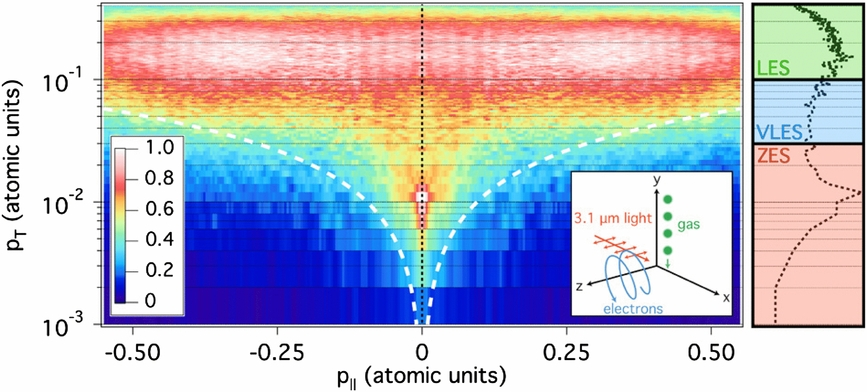
\includegraphics[scale=1]{6-LES/Figures/figure6D.jpg}
  \caption[
  Observation of (Near-)Zero Energy Structures by Pullen et al.
  ]{
  Low-energy momentum distribution (in linear and log scale for the longitudinal and transverse momentum, respectively) for unaligned molecular nitrogen ionized by a $\SI{3.1}{\micro\meter}$ field at $\SI{e14}{\watt/\centi\meter^2}$~\cite{ pullen_kinematically_2014}, showing peaks and structures at the LES and VLES ranges, highlighted in the side inset, and an additional peak at even lower photoelectron energy.
  Figure excerpted from \citer{pullen_kinematically_2014}.
  }
\label{f6-pullen-original-full-spectrum}
\end{figure}
\copyrightfootnote{
\reffig{f6-pullen-original-full-spectrum} © IOP Publishing. Reproduced with permission. All rights reserved.
}
%% Copyright note is temporary pending IOP reply.






Upon its discovery, this peak was dubbed a Zero-Energy Structure (ZES), since the center of the peak is consistent with zero to within the available experimental precision both at the time of its discovery~\cite{pullen_kinematically_2014} and to date. However, as we shall see below, there is reason to suspect that the center may not be at zero but only close to it, so a much better name for the structure is Near-Zero-Energy Structure (NZES), which we will use throughout and as a synonym for ZES, and which better reflects the fact that in physics it is rather rare to have values exactly at zero instead of merely consistent with it.


The angle-resolved photoelectron spectra of Refs.~\cite{dura_ionization_2013} and \cite{pullen_kinematically_2014}, as well as later publications, have several interesting features worth emphasizing. The first is the relatively trivial observation that, because of the volume element of the cylindrical coordinates being employed, it is naturally harder for electrons to fall exactly on-axis (at $\pt=0$) and on the volume element around it, which explains the detection probability on the lower part of \reffig{f6-pullen-original-full-spectrum}. This effect is also responsible for making the NZES form as a distinct spot separate from the axis, even though the structure is consistent with having its centre at the origin of the momentum plane; it also makes the high detection counts at the NZES spot, and above it, all the more remarkably high, particularly when compared to similar~$\pt$ at~higher $\pp$.


The second important feature is that, in experiments performed in Reaction Microscope detector configuration, the VLES peak which would be expected at the $\SI{100}{\milli\electronvolt}$ range essentially vanishes. This is due to the fact that the previous observations were performed using time-of-flight (TOF) electron spectrometers~\cite{VLES_initial, VLES_characterization}, which have a very narrow acceptance cone of about $\SI{6}{\degree}$ centred on the laser polarization, and this leaves out a large fraction of the produced photoelectrons and the features in their distribution. This acceptance cone is shown as a dashed white line in \reffig{f6-pullen-original-full-spectrum}, and the electrons shown in Figs.~\ref{f6-quan-original-figure} and \ref{f6-wu-original-figure} all originate \textit{below} the dashed line. On the other hand, if the full three-dimensional data is post-selected to only the electrons within that acceptance angle, the VLES peaks reappear~\cite[p.~5]{pullen_kinematically_2014}. This means, then, that the VLES as originally reported are not quite an experimental artefact, but the initial detections are certainly only a very partial look at much richer structures.

Finally, it is important to remark that the upper limit of the electron spectrum at around $\pt\approx\SI{0.3}{\au}$ is an artefact of the detection apparatus, which is configured for low-energy electrons at high resolution, and therefore leaves out higher momenta.


The first of these features also points out an important aspect of the photoelectron spectra in the low-energy region, which is the fact that the transverse momentum distribution will vary wildly for different longitudinal momenta. Indeed, the experimental transverse distributions, shown in \reffig{f6-pullen-original-transverse-spectrum}, show large differences in photoelectron spectra taken over broad $\pp$ ranges and the slice at $|\pp|<\SI{0.02}{\au}$, where the NZES congregates. In this view, the NZES is clearly visible as a spike of width $\Delta\pt\approx\SI{0.05}{\au}$ (though this also includes some electrons from the V-like structure of the VLES).





\begin{figure}[hb]
  \centering
  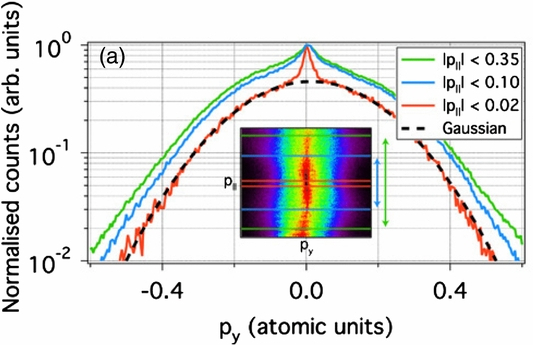
\includegraphics[scale=1.2]{6-LES/Figures/figure6E.jpg}
  \caption[
  Experimental transverse photoelectron momentum spectra at different longitudinal momenta, observed by Pullen et al.]{
  Transverse photoelectron momentum distributions at different longitudinal momentum for the data displayed in \reffig{f6-pullen-original-full-spectrum}. Integrating over a broad $\pp$ range yields a cusp with a smooth drop-off, whereas a smaller range around zero longitudinal momentum brings out a sharp peak at the origin coming out of a gaussian background.
  Figure excerpted from \citer{pullen_kinematically_2014}.
  }
\label{f6-pullen-original-transverse-spectrum}
\end{figure}
\copyrightfootnote{
\reffig{f6-pullen-original-transverse-spectrum} © IOP Publishing. Reproduced with permission. All rights reserved.
}
%% Copyright note is temporary pending IOP reply.
%
%
\copyrightfootnote{
\reffig{f6-wolter-original-figure} reprinted with permission from B. Wolter et al., {%
\hypersetup{urlcolor=black}%
\href{http://dx.doi.org/10.1103/PhysRevA.90.063424}{%
\emph{Phys.\ Rev.\ A} \textbf{90}, 036424 (2014)}. %
© 2014 by the American Physical Society.
}
}
%% As per APS T&Cs



\begin{figure}[h!t]
  \vspace{2mm}
  \centering
  \subfloat{\label{f6-wolter-original-figure-a}}
  \subfloat{\label{f6-wolter-original-figure-b}}
  \subfloat{\label{f6-wolter-original-figure-c}}
  \subfloat{\label{f6-wolter-original-figure-d}}
  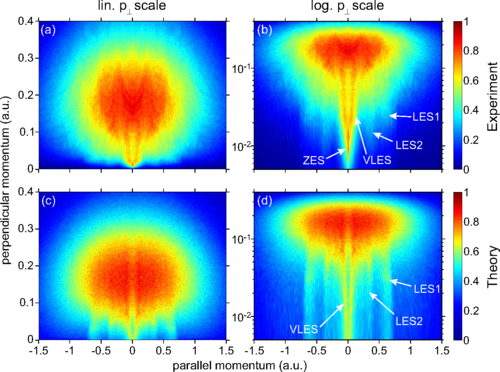
\includegraphics[scale=0.7]{6-LES/Figures/figure6F.png}
  \caption[
  Measured and CTMC high-resolution photoelectron momentum maps showing LES, VLES and ZES structures, observed by Wolter et al.
  ]{
  Measured momentum maps for the ionization of argon in a $\SI{3.1}{\micro\meter}$ 6.5-cycle pulse at $\SI{9e13}{\watt/\centi\meter^2}$ \cite{ZES_paper}, showing the V-shaped VLES and the NZES peak, as well as two distinct LES structures, in both linear (left) and logarithmic (right) transverse momentum scales. Most of the features are reasonably well reproduced by a classical trajectory Monte Carlo simulation (bottom row).
  Figure excerpted from \citer{ZES_paper}.
  }
\label{f6-wolter-original-figure}
\end{figure}


\pagebreak




Since the original detection of the NZES, several improvements in the measurement stability and resolution have enabled better characterizations of the photoelectron distribution structures over momentum space~\cite{ZES_paper}. This includes a series of additional LES peaks, each with a distinct structure at relatively constant transverse momentum, and with progressively smaller longitudinal position, as shown in \reffig{f6-wolter-original-figure} and subsequently refined \cite{Wolter_PRX} as shown in \reffig{f6-wolter-prx-original-figure}. These features were indeed expected, as we shall show below, coming from different members of a family of trajectories.




\begin{figure}[htb]
  \centering
  \subfloat{\label{f6-wolter-prx-original-figure-a}}
  \subfloat{\label{f6-wolter-prx-original-figure-b}}
  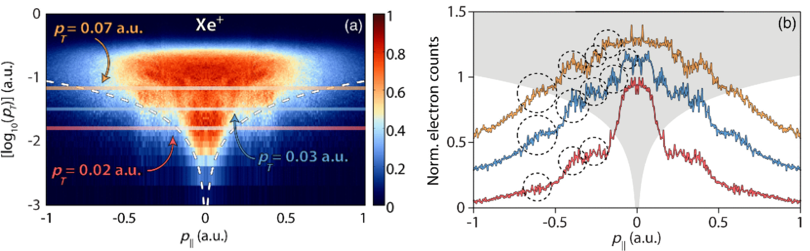
\includegraphics[width=\textwidth]{6-LES/Figures/figure6G.png}
  \caption[
  Measured photoelectron momentum map showing multiple members of the LES series, observed by Wolter et al.
  ]{
  Momentum map \protect\subref{f6-wolter-prx-original-figure-a} for the ionization of xenon in a $\SI{3.1}{\micro\meter}$ pulse of intensity $\SI{4e13}{\watt/\centi\meter^2}$ \cite{Wolter_PRX}, showing clear LES but slightly muddled VLES V-shape and NZES peak. Line-outs at several different transverse momenta $\pt$ produce longitudinal profiles with distinct LES peaks shown inside dashed circles in \protect\subref{f6-wolter-prx-original-figure-b}. The gray region in \protect\subref{f6-wolter-prx-original-figure-b} is a rough approximation of the features excluded by the TOF acceptance cone, shown as the white dashed line in \protect\subref{f6-wolter-prx-original-figure-a} as in \reffig{f6-pullen-original-full-spectrum}. The data have been symmetrized about $\pp=0$. 
  Figure excerpted from \citer{Wolter_PRX}.
  }
\label{f6-wolter-prx-original-figure}
\end{figure}
\copyrightfootnote{
\reffig{f6-wolter-prx-original-figure} reused under its {%
\hypersetup{urlcolor=black}%
\href{https://creativecommons.org/licenses/by/3.0/}{CC BY licence}, from B. Wolter et al., 
\href{http://dx.doi.org/10.1103/PhysRevX.5.021034}{%
\emph{Phys.\ Rev.\ X} \textbf{5}, 021034 (2015)}. %
}
}

As of this writing, the measurements in \citer{Wolter_PRX}, as showcased for example in \reffig{f6-wolter-prx-original-figure}, essentially represent the state of the art in the experimental observations of the low-energy region of above-threshold ionization in mid-IR fields. In particular, there is clear evidence of multiple LES features, well-resolved V-shape VLES structures, and strong NZES peaks, though the information on the latter is limited mostly to only its presence.




\subsection{Theoretical explanations for low-energy structures}
\label{sec:LES-theory}
In terms of the available theoretical explanations for the structures in the low-energy region of mid-{IR} strong-field ionization, the field is rather more varied and offers a less linear story. There is a general consensus that the LES is caused by the Coulomb potential acting on the mostly classical motion of the electron, and specifically centred on soft recollisions. On the other hand, there are several alternative mechanisms to go from this class of trajectories to peaks in the photoelectron spectrum.


%%% TDSE

As we saw earlier, from its initial detection the LES was reproducible from within TDSE simulations~\cite{blaga_original_LES,catoire_angular-distributions_2009}, and this has been carried forward with TDSE calculations showing the VLES, in their original sense as a single peak under a constrained acceptance angle~\cite{VLES_characterization}. In addition to this there have been some attempts at further exploration of the low-energy region within the TDSE~\cite{telnov_TDSE_with_and_without_Coulomb, lemell_classicalquantum_2013}, but generally the consensus is that those features, and most markedly the LES, are well explained by the TDSE and therefore captured completely by the single-atom Schrödinger equation. Unfortunately, this yields relatively little insight on the origin of the structures, and most of the effort has been directed at building simplified models that explain the structures.


%%% Overview

These efforts largely fall along three lines of inquiry. On the classical side, one can study the global properties of the classical propagation map, and one can also use statistical Monte Carlo methods to predict photoelectron spectra. On a more explicitly quantum side, there is the Coulomb-Corrected SFA (CCFA), which we discussed in the Introduction and in chapter~\ref{chap:quantum-orbits}, and which embeds the classical trajectory dynamics directly within the quantum SFA framework. Finally, a class of methods known as Improved SFA (ISFA), include a single term of interaction with the core in a Born series and then perform an expanded SFA treatment. This varied set of methods generally agrees on the causes for the LES, in terms of the classes trajectories involved, but they provide multiple interpretations for how those trajectories translate into peaks in photoelectron spectra.	


%%% CTMC

One prominent feature of this set of explanations is that much of the structure that is present can be explained rather well using only classical trajectories, building on electron populations that are built up throughout the laser cycle as ionization bursts given by the quasi-static ADK tunnelling probability. This is known as the Classical Trajectory Monte Carlo (CTMC) method: a large number of electron trajectories are randomly generated, weighed by the ADK rate, and they are then propagated until the end of the pulse using the newtonian equation of motion in the laser field plus the (effective) ionic potential. In essence, the Schrödinger dynamics of the photoelectron are replaced by Liouvillian statistical mechanics with an ADK source term.

This approach is able to reproduce the LES and VLES peaks \cite{CTMC1, CTMC2, zhi_Coulomb-LES_2014, lemell_lowenergy_2012} and, moreover, it is able to dissect those structures by selecting the electrons that do end up inside the relevant structures and exploring their characteristics in terms of ionization time~\cite{VLES_characterization, zhi_Coulomb-LES_2014}, angular momentum~\cite{lemell_lowenergy_2012, lemell_classicalquantum_2013}, and overall shape~\cite{lemell_classicalquantum_2013, xia_near-zero-energy_2015}, a level of access into the internal details of the components of a simulation that is denied to TDSE calculations.



\newlength{\figuresixHheight}
\setlength{\figuresixHheight}{5.5cm}
\begin{figure}[hb]
  \centering
  \subfloat{\label{f6-xia-original-figure-a}}
  \subfloat{\label{f6-xia-original-figure-b}}
  \subfloat{\label{f6-xia-original-figure-c}}
  \subfloat{\label{f6-xia-original-figure-d}}
  \subfloat{\label{f6-xia-original-figure-e}}
  \subfloat{\label{f6-xia-original-figure-f}}
  \subfloat{\label{f6-xia-original-figure-g}}
  \subfloat{\label{f6-xia-original-figure-h}}
  \subfloat{\label{f6-xia-original-figure-i}}
  \subfloat{\label{f6-xia-original-figure-j}}
  \subfloat{\label{f6-xia-original-figure-k}}
  \subfloat{\label{f6-xia-original-figure-l}}
  \begin{tabular}{ccc}
  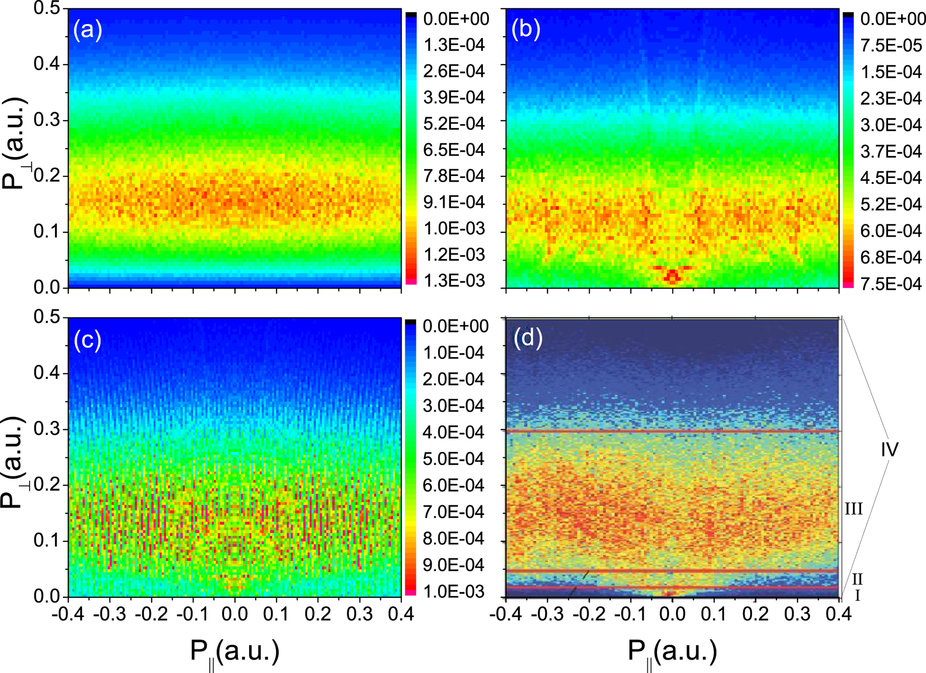
\includegraphics[height=\figuresixHheight]{6-LES/Figures/figure6Ha.png} 
  & \hspace{0mm} &
  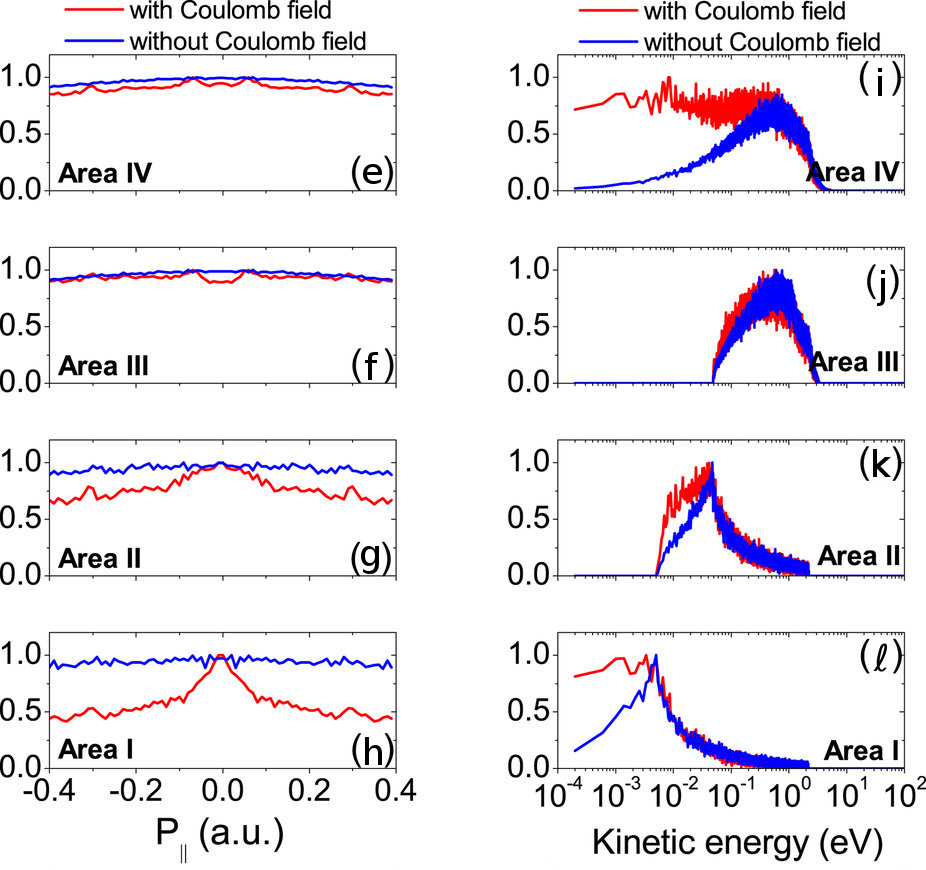
\includegraphics[height=\figuresixHheight]{6-LES/Figures/figure6Hb.png}
  \end{tabular}
  \caption[
  CTMC simulations of VLES V-shaped structure and NZES-like peak, performed by Q.Z. Xia et al.
  ]{
  Photoelectron momenta for argon ionized by a $\SI{e14}{\watt/\centi\meter^2}$ laser at $\SI{3.1}{\micro\meter}$, as obtained via CTMC simulations using \protect\subref{f6-xia-original-figure-a} no Coulomb potential, \protect\subref{f6-xia-original-figure-b} the full Coulomb interaction, and \protect\subref{f6-xia-original-figure-c} Coulomb interactions with a trajectory interference term, as compared to the experimental data from \citer{dura_ionization_2013} shown in \protect\subref{f6-xia-original-figure-d}. The results can be divided into zones and explored with the Coulomb interaction turned on and off, as shown for the different zones of \protect\subref{f6-xia-original-figure-d} over longitudinal momentum \protect\subref{f6-xia-original-figure-e}-\protect\subref{f6-xia-original-figure-h} and kinetic energy \protect\subref{f6-xia-original-figure-i}-\protect\subref{f6-xia-original-figure-l}.
  Figure excerpted from \citer{xia_near-zero-energy_2015}.
  }
\label{f6-xia-original-figure}
\end{figure}
\copyrightfootnote{
\reffig{f6-xia-original-figure} adapted (labels (e-l) shifted for clarity), under its {%
\hypersetup{urlcolor=black}%
\href{https://creativecommons.org/licenses/by/3.0/}{CC BY licence}, from Q.Z. Xia et al., 
\href{http://dx.doi.org/10.1038/srep11473}{%
\emph{Sci.\ Rep.} \textbf{5}, 11473 (2015)}. %
}
}
%%% To do: change package from subfigure to subfig, add \subref* to the e-h and i-l references in the caption.



Further, CTMC simulations can also reproduce much of the V-shaped VLES and a NZES-like peak in the photoelectron momentum spectrum~\cite{xia_near-zero-energy_2015}, shown in \reffig{f6-xia-original-figure-b}, and remarkably close to the equivalent experimental result from \citer{dura_ionization_2013} shown in \reffig{f6-xia-original-figure-d}. In addition to this, CTMC results have conclusively shown that the Coulomb field of the remaining ion is essential to the emergence of LES and related structures~\cite{zhi_Coulomb-LES_2014, xia_near-zero-energy_2015}, as shown for example in \reffig{f6-xia-original-figure-a}: here the ionic potential is completely ignored after the ADK tunnelling stage, completely eliminating the features of \reffig{f6-xia-original-figure-b}. (Similar differences are exhibited in \reffig{f6-xia-original-figure-e}-\subref{f6-xia-original-figure-l}.)



In addition to the statistical look provided by the CTMC method, the classical mechanics of post-tunnelling electrons can also provide deeper, structural looks at what causes the LES peaks, by examining the dynamical maps of the newtonian evolution, from the conditions after ionization to the electron momenta after several laser periods~\cite{Rost_PRL, Rost_JPhysB}. Under this lens, the LES peak is caused by dynamical focusing: the bunching together of electrons that come from a wide array of initial conditions into a relatively small interval, as shown in \reffig{f6-kastner-dynamical-focusing}.





\begin{figure}[htbp]
  \centering
  \subfloat{\label{f6-kastner-original-figure-a}}
  \subfloat{\label{f6-kastner-original-figure-b}}
  \subfloat{\label{f6-kastner-original-figure-c}}
  \subfloat{\label{f6-kastner-original-figure-d}}
  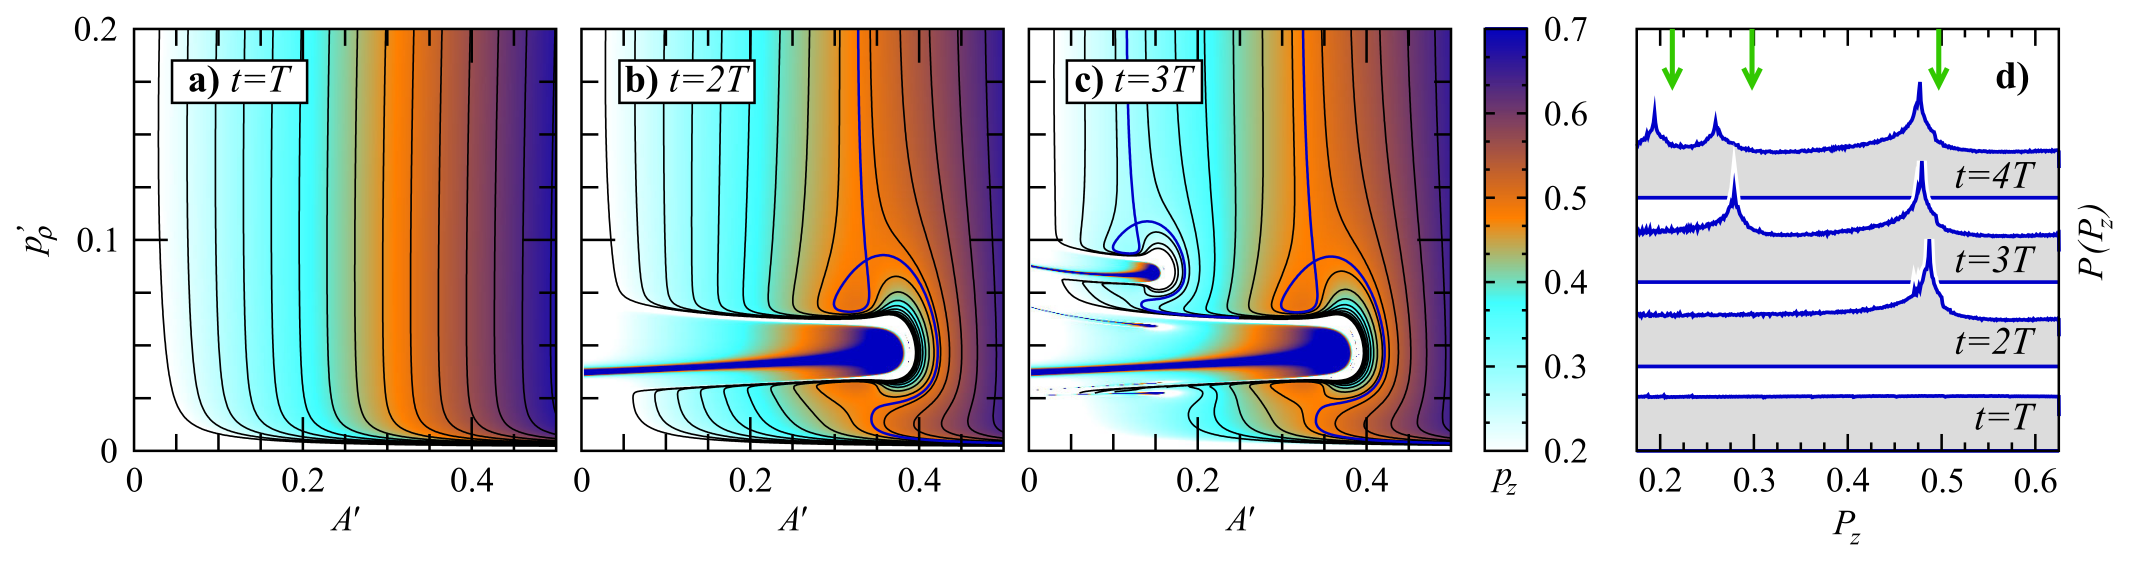
\includegraphics[width=\textwidth]{6-LES/Figures/figure6I.png}
  \caption[
  Dynamical maps for classical trajectories showing `finger'-like structures and the associated photoelectron bunching, as calculated by A. Kästner~et~al.
  ]{
  Dynamical maps for a classical electron released into a monochromatic field $A'=A_0\sin(\omega t)$ under the influence of a Coulomb potential~\cite{Rost_PRL}. The electron is released with ADK rates at a time $t'$, indexed by the vector potential $A'$ at ionization, with initial transverse momentum $p'_\rho$ and zero transverse velocity. The colour scale shows the electron longitudinal momentum $p_z$ as a function of the initial conditions at one \protect\subref{f6-kastner-original-figure-a}, two \protect\subref{f6-kastner-original-figure-b} and three \protect\subref{f6-kastner-original-figure-c} laser periods after ionization. The `fingers' in \protect\subref{f6-kastner-original-figure-b} and \protect\subref{f6-kastner-original-figure-c} represent depletion caused by a soft recollision, and this is accompanied by peaks in the spectrum \protect\subref{f6-kastner-original-figure-d} caused by dynamical focusing: the crossed, looping contours around the saddle points of $p_z(p_\rho',A')$, where the electrons congregate.
  Figure excerpted from \citer{Rost_PRL}.
  }
\label{f6-kastner-dynamical-focusing}
\end{figure}
\copyrightfootnote{
\reffig{f6-kastner-dynamical-focusing} reprinted with permission from A. Kästner et al., {%
\hypersetup{urlcolor=black}%
\href{http://dx.doi.org/10.1103/PhysRevLett.108.033201}{%
\emph{Phys.\ Rev.\ Lett.} \textbf{108}, 033201 (2012)}. %
©~2012 by the American Physical Society.
}
}
%% As per APS T&Cs


This occurs at momenta close to (but not exactly at) the soft-recollision momenta, for which the electron returns to the core, $\vbr(t_r) \approx 0$, for a close interaction with the ion, and moreover it does so with a very low velocity, $\vbv(t_r)\approx 0$, as shown in \reffig{f6-rost-soft-recollisions}. For the full classical trajectories, the soft recollision itself is often `burned' out of the spectrum and sent to radically different momenta, shown as the `fingers' of Figs.~\ref{f6-kastner-original-figure-b} and \subref{f6-kastner-original-figure-c}, but the strong effect on the momentum-momentum mapping causes spots nearby to fold a flat initial distribution into a peak at the zeroes of the derivative of the mapping.


Moreover, once this cause is recognized, it is easy to see that the soft recollisions of \reffig{f6-rost-soft-recollisions} come in multiple types. The principal trajectory type, which causes the main LES peak, has a soft recollision at one and a half periods after it is ionized: it swings past the ion once (at a velocity too high to be meaningfully deflected) and then has a soft recollision on the turning point of its next backwards swing, as shown by the green curve~of~\reffig{f6-rost-soft-recollisions}.



\begin{figure}[b!]
\centering
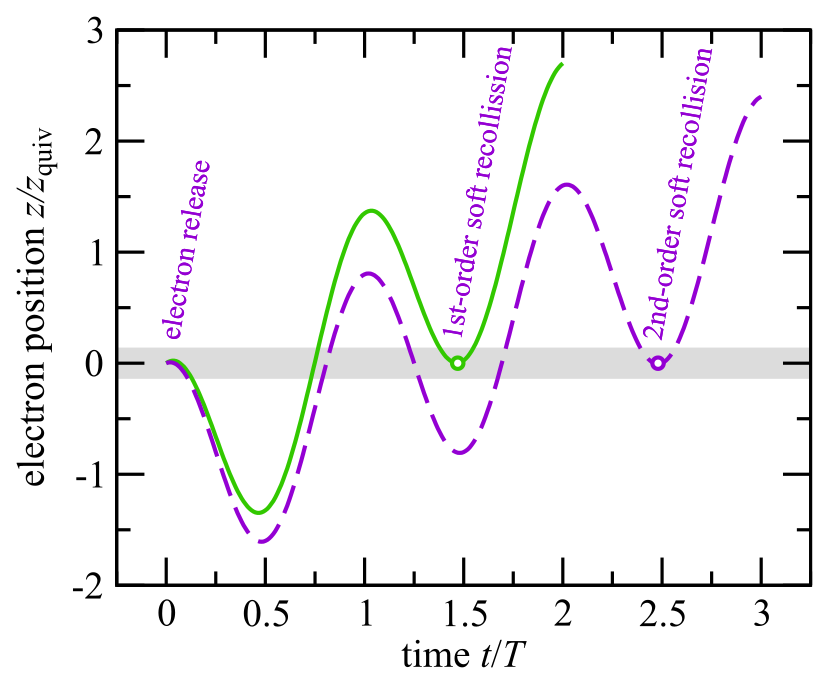
\includegraphics[scale=1]{6-LES/Figures/figure6J.png}
  \caption[
  Soft recollisions as originally presented by A. Kästner et al.
  ]{
  Soft recollisions are trajectories where the electron returns to the vicinity of its parent ion with very small velocity, near a turning point. This can be after a single pass (green curve) or after two (purple curve) or more passes, forming a family of trajectories at different final momenta.
  Figure excerpted from \citer{Rost_JPhysB}.
  }
\label{f6-rost-soft-recollisions}
\end{figure}
\copyrightfootnote{
\reffig{f6-rost-soft-recollisions} © IOP Publishing. Reproduced with permission. All rights reserved.
}
%% Copyright note is temporary pending IOP reply.




It is possible, however, for trajectories to have a soft recollision later on in the cycle, like the purple, dashed curve, which spends two periods oscillating at relatively large distances from the origin (and, again, passing the ion too quickly to get too deflected), and having a soft recollision on its second backwards turning point. This then generates a series of trajectories starting with the LES peak and going to lower and lower momentum (which we will explore in more depth in section~\ref{sec:classical-soft-recollisions}), causing the series of peaks seen in \reffig{f6-kastner-original-figure-d}; these predicted peaks do appear in experimental spectra~\cite{ZES_paper, Wolter_PRX}, as discussed above, and they are visible in the experimental results shown in Figs.~\ref{f6-wolter-original-figure} and \ref{f6-wolter-prx-original-figure}.

%
%
%\begin{figure}[t]
%\centering
%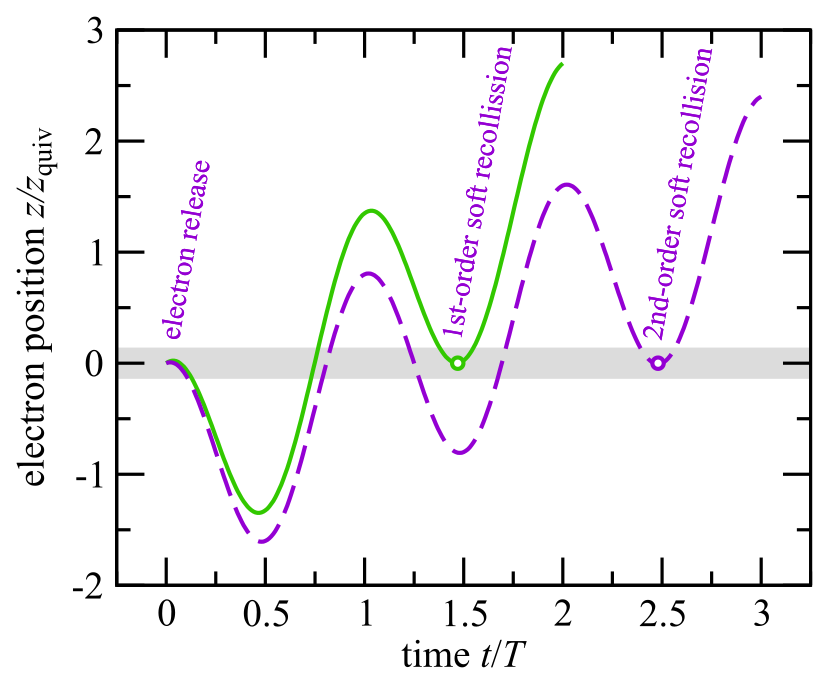
\includegraphics[scale=1]{6-LES/Figures/figure6J.png}
%  \caption[
%  Soft recollisions as originally presented by A. Kästner et al.
%  ]{
%  Soft recollisions are trajectories where the electron returns to the vicinity of its parent ion with very small velocity, near a turning point. This can be after a single pass (green curve) or after two (purple curve) or more passes, forming a family of trajectories at different final momenta.
%  Figure excerpted from \citer{Rost_JPhysB}.
%  }
%\label{f6-rost-soft-recollisions}
%\end{figure}
%\copyrightfootnote{
%\reffig{f6-rost-soft-recollisions} © IOP Publishing. Reproduced with permission. All rights reserved.
%}
%%% Copyright note is temporary pending IOP reply.


Going some way beyond this analysis, the dynamical map of the full Coulomb-plus-laser trajectories, i.e. the mapping from the momentum at ionization to the momentum after one laser period and beyond, is a rather complicated quantity~\cite[cf.][Fig.~7]{Becker_rescattering}, but if examined in detail it can show some very interesting regularities, shown in~\reffig{f6-kelvich-dynamical-map}.


\begin{figure}[htb]
  \centering
  \subfloat{\label{f6-kelvich-original-figure-a}}
  \subfloat{\label{f6-kelvich-original-figure-b}}
  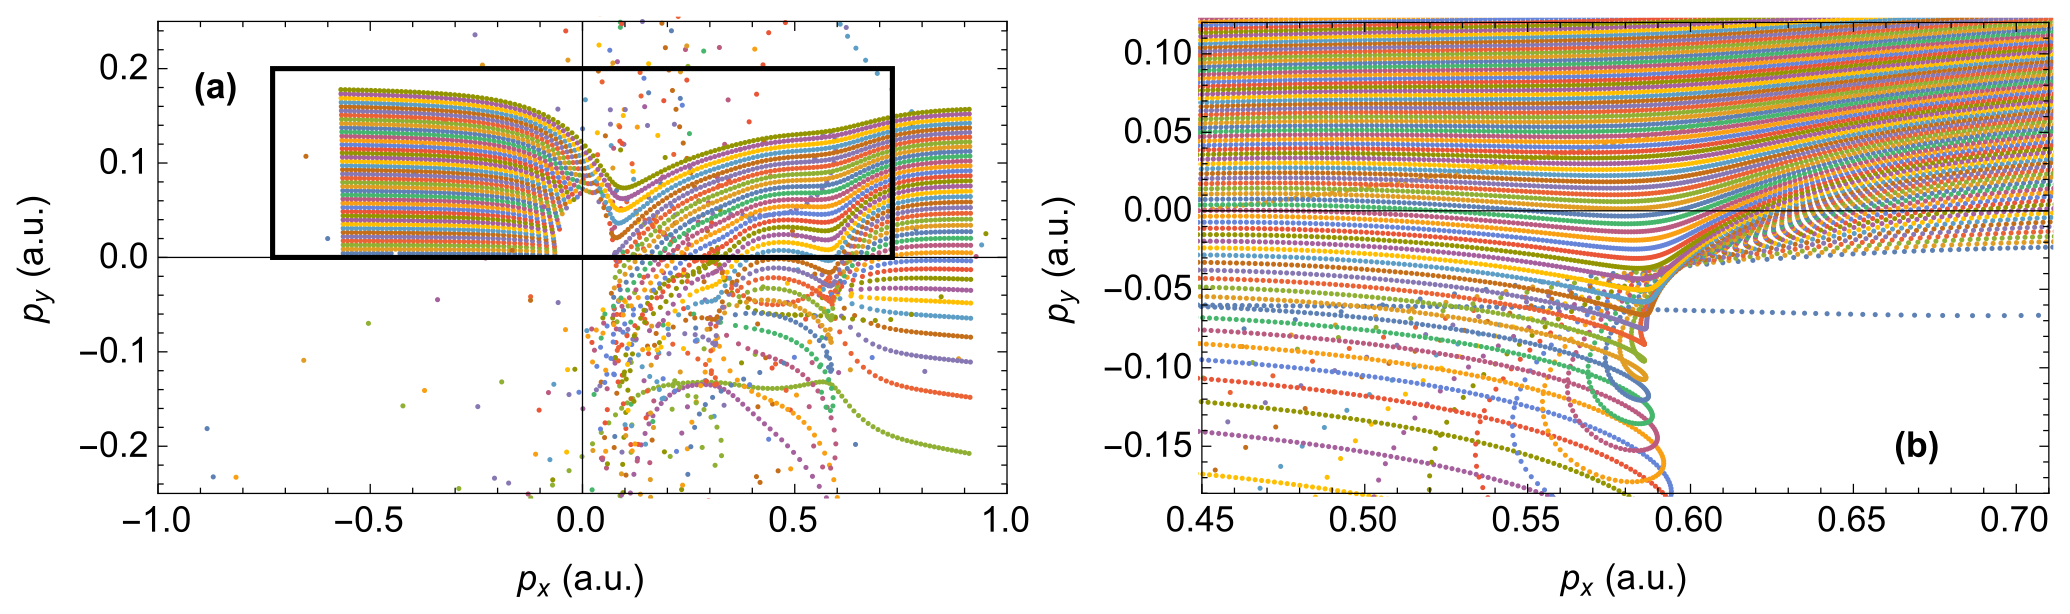
\includegraphics[width=392pt]{6-LES/Figures/figure6K.png}
  \caption[
  High-resolution dynamical map of full classical photoelectron trajectories, showing LES bunching as the result of a caustic in the dynamical map, as calculated by S.A. Kelvich et al.
  ]{
  Dynamical map of electrons ionized from argon by a $\SI{1.5e14}{\watt/\centi\meter^2}$ field at $\SI{2}{\micro\meter}$, taking a regular grid in momentum space to a complicated shape~\cite{kelvich_coulomb-focusing_2015}. The decrease in width compared to the non-Coulomb case (black rectangle) showcases the known Coulomb focusing, but near the soft recollision at $p_x\approx\SI{0.61}{\au}$ the trajectories are sent to an opposite transverse momentum $p_y$, forming the caustic shown in \protect\subref{f6-kelvich-original-figure-b}, which then accumulates electrons to form an LES peak in the photoelectron spectrum.
  Figure excerpted from \citer{kelvich_coulomb-focusing_2015}.
  }
\label{f6-kelvich-dynamical-map}
\end{figure}
\copyrightfootnote{
\reffig{f6-kelvich-dynamical-map} reprinted with permission from S.\ A. Kelvich et al., {%
\hypersetup{urlcolor=black}%
\href{http://dx.doi.org/10.1103/PhysRevA.93.033411}{\emph{Phys.\ Rev.\ A} \textbf{93}, 033411 (2016)}. %
©~2016 by the American Physical Society.
}
}
%% As per APS T&Cs

It is quite clear, from the detailed mapping, that some regions exhibit chaotic dynamics~\cite{chaotic_dynamics} (which show up as the burned-out hole near the origin, where the electrons are scattered away), but there are also large regions of regularity. For instance, the main LES is clearly visible as the result of a caustic induced by the Coulomb potential, shown in \reffig{f6-kelvich-original-figure-b}, which then causes the electron bunching at those energies.





%%% CCSFA
These results, then, show that classical trajectories capture much of the dynamics of the LES, but in the end the ionization process is quantum mechanical, and it is worthwhile to look for methods that explicitly include the quantum mechanical aspects of the problem. This is, essentially, the Coulomb-corrected SFA (CCFSA) approach which we discussed in section~\ref{sec:emergence-of-complex-trajectories}, and which was developed in Refs.~\citealp{CCSFA_initial_short} and~\citealp{ CCSFA_initial_full} for use in problems like sub-barrier Coulomb effects in tunnel ionization~\cite{TCSFA_sub_barrier}, which it can do quite successfully within the conceptual constraints we detailed in section~\ref{sec:emergence-of-complex-trajectories}.

When applied to the LES, the CCSFA method produces angular distributions somewhat different to the ones obtained by classical-trajectory CTMC methods~\cite{ yan_TCSFA_caustics}, but it does provide a good match to the TDSE distributions, as shown in \reffig{f6-yan-original-figure}, which in principle describes the microscopic response better, prior to the washing out of interference fringes by focal averaging effects. As such, the CCSFA results form a useful bridge, connecting the full Schrödinger equation on one side with the classical understanding in terms of soft recollisions on the other.




\begin{figure}[htb]
  \centering
  \subfloat{\label{f6-yan-original-figure-a}}
  \subfloat{\label{f6-yan-original-figure-b}}
  \subfloat{\label{f6-yan-original-figure-c}}
  \subfloat{\label{f6-yan-original-figure-d}}
  \subfloat{\label{f6-yan-original-figure-e}}
  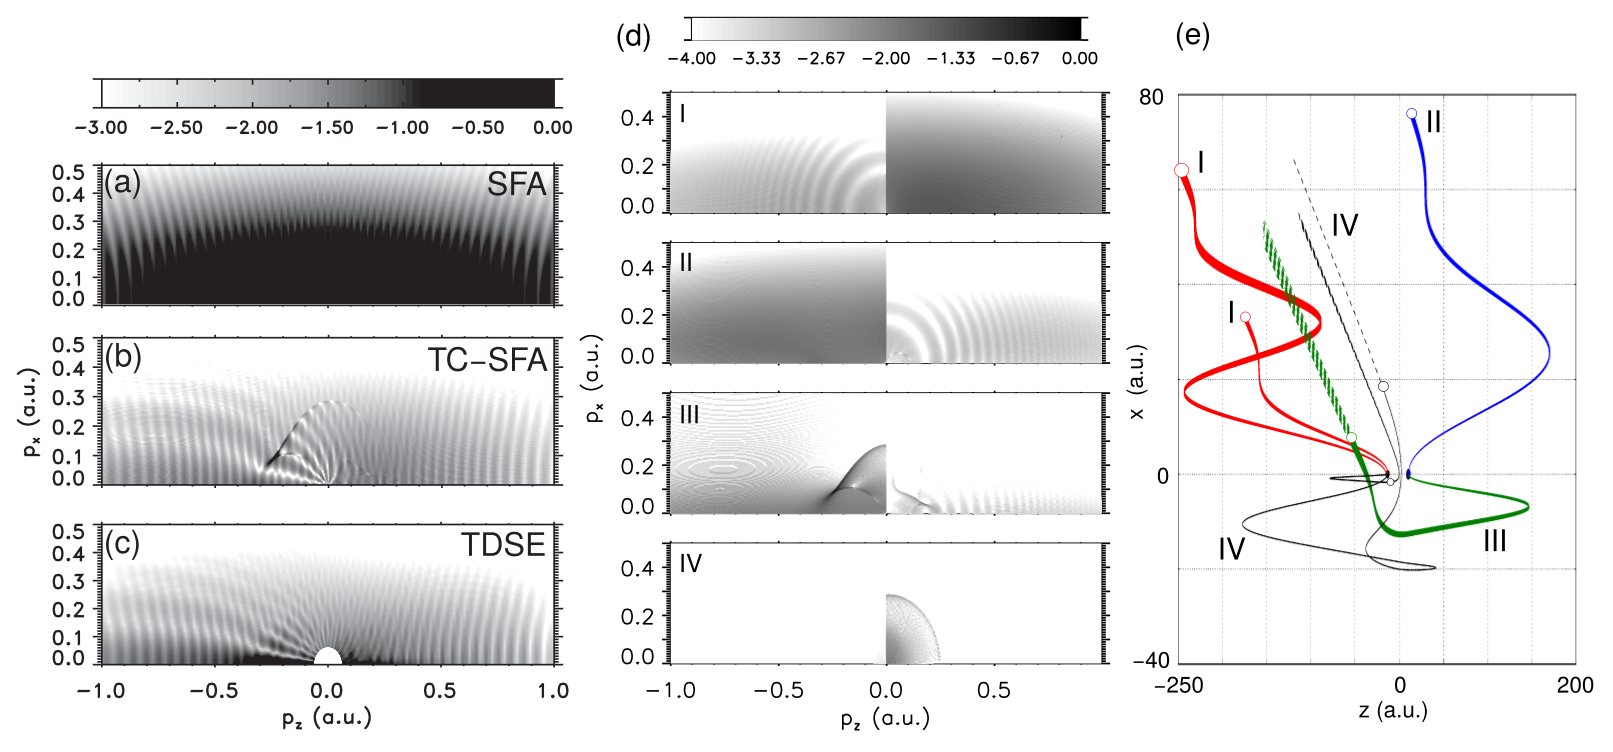
\includegraphics[width=\textwidth]{6-LES/Figures/figure6L.png}
  \caption[
  CCSFA analysis of the Low-Energy Structures, as performed by T.-M. Yan~et~al.
  ]{
  Photoelectron momentum distributions from argon ionized by a $\SI{2}{\micro\meter}$ field at $\SI{e12}{\watt/\centi\meter^2}$~\cite{ yan_TCSFA_caustics}, via standard SFA \protect\subref{f6-yan-original-figure-a}, a full TDSE simulation~\protect\subref{f6-yan-original-figure-c}, and a CCSFA~(here named TC-SFA) calculation~\protect\subref{f6-yan-original-figure-b}. The CCSFA result provides a good match to the full TDSE, while still providing an intuitive trajectory picture. Specifically, the `cut' at the LES range in \protect\subref{f6-yan-original-figure-b} can be directly associated with a caustic, coming from trajectory type III as per \protect\subref{f6-yan-original-figure-e}, where the electron approaches the ion at low speed, changing the sign of its transverse momentum.
  Figure excerpted from \citer{yan_TCSFA_caustics}.
  }
\label{f6-yan-original-figure}
\end{figure}
\copyrightfootnote{
\reffig{f6-yan-original-figure} reprinted with permission from T.-M. Yan et al., {%
\hypersetup{urlcolor=black}%
\href{http://dx.doi.org/10.1103/PhysRevLett.105.253002}{%
\emph{Phys.\ Rev.\ Lett.} \textbf{105}, 253002 (2010)}. %
©~2010 by the American Physical Society. Labels (d,\,e) shifted for clarity.
}
}
%% As per APS T&Cs





%%% ISFA
In addition to this, it is also possible to do an even deeper quantum approach, by augmenting the normal SFA with a single formal quantum scattering on the ionic potential. This approach, known as the Improved SFA (ISFA), builds a Born series in the Coulomb potential in much the same way that we performed a perturbative expansion with respect to the electron correlation interaction potential $V_{ee}^m$ in chapter~\ref{chap:R-matrix}. It was originally developed to deal with a large plateau of high-energy electrons (between $2U_p$ and $10U_p$) in above-threshold ionization~\cite{goreslavskii_ISFA-standard_1998, milosevic_ISFA-standard_2007}, and it has been very successful there, but it can also be applied to forward scattering at low velocities.

In the LES context, then, the ISFA method can describe the LES peaks~\cite{ Becker_rescattering, Becker_Milosevic_quantum_orbits, Milosevic_scattering_large, Milosevic_reexamination, becker_milosevic_unified_2016}, which appear as a result of forward scattering with the Coulomb core at low energies. This had originally been neglected, because the direct pathway (without rescattering) was deemed dominant at low energies, but the large Coulomb scattering cross section in the forward direction makes up for the difference. 

Moreover, the forward scattering within ISFA can also be used to explain the V-shaped VLES~\cite{Becker_Milosevic_quantum_orbits, becker_ATI-low-energy_2015}, where it shows as the confluence of the locus of several types of forward-scattered quantum orbits, as shown in \reffig{f6-becker-circles-original-figure}, with the predicted spectrum providing a good match to the experimental observations of \reffig{f6-wolter-original-figure}.


\newlength{\figuresixMheight}
\setlength{\figuresixMheight}{6cm}
\begin{figure}[htb]
  \centering
  \subfloat{\label{f6-becker-circles-original-figure-a}}
  \subfloat{\label{f6-becker-circles-original-figure-b}}
  \begin{tabular}{ccc}
  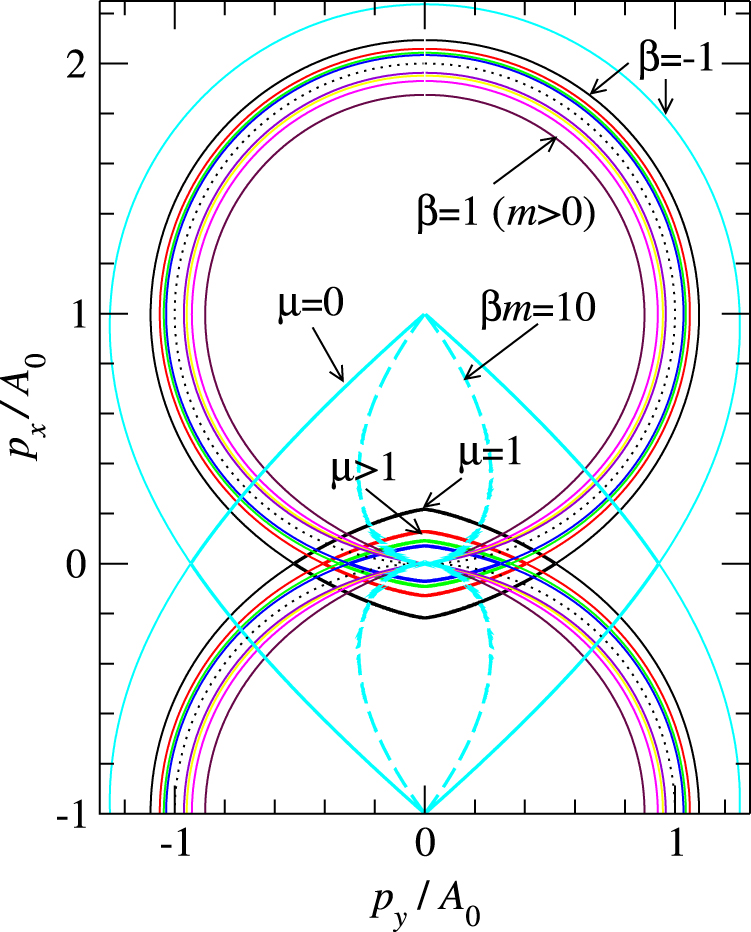
\includegraphics[height=\figuresixMheight]{6-LES/Figures/figure6Ma.jpg}
  & & 
  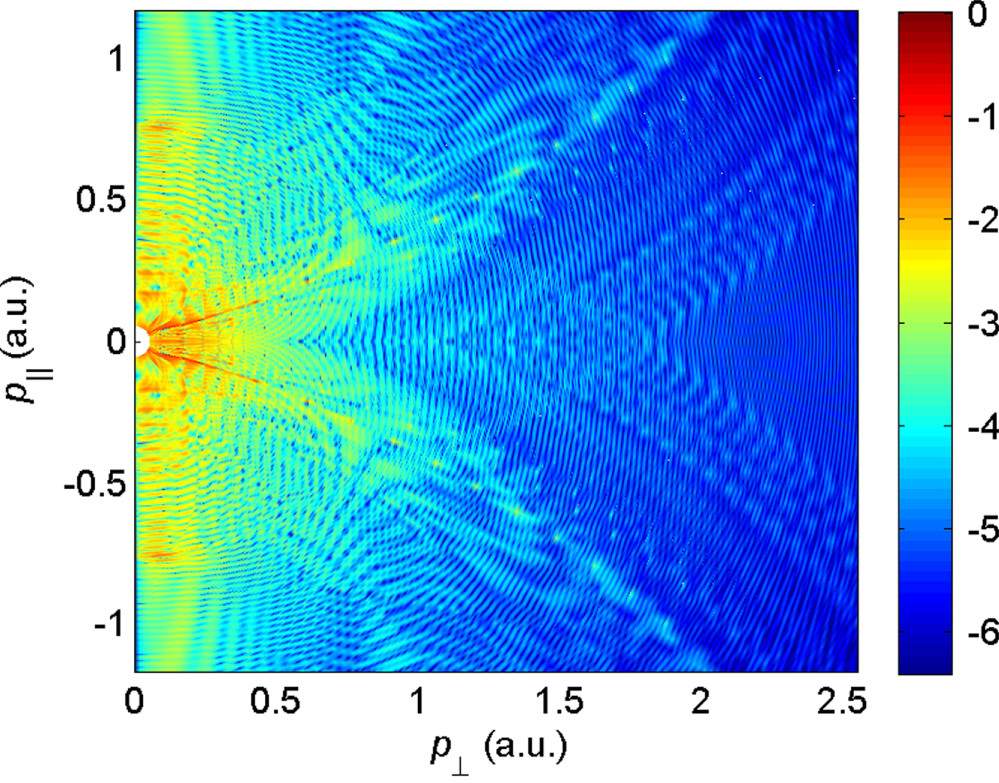
\includegraphics[height=\figuresixMheight]{6-LES/Figures/figure6Mb.jpg}
  \end{tabular}
  \caption[
  Emergence of the VLES V-shape from forward-scattered quantum orbits within the ISFA formalism, as presented by W. Becker et al.
  ]{
  Emergence of the VLES V-shape from forward-scattered quantum orbits within the ISFA formalism~\cite{becker_ATI-low-energy_2015}. Here multiple quantum orbits (with different starting times, indexed by $\beta$, $\mu$ and $m$) form contributions with different loci, which are essentially universal up to the field momentum scale $A_0=F/\omega$. The intersection of the circular loci at the origin then gives rise to the V shape, as shown in the predicted spectrum \protect\subref{f6-becker-circles-original-figure-b} for argon in a $\SI{3.1}{\micro\meter}$ field at $\SI{9e13}{\watt/\centi\meter^2}$ as in \citer{ZES_paper}. Figure excerpted from~\citer{ becker_ATI-low-energy_2015}.
  }
\label{f6-becker-circles-original-figure}
\end{figure}
\copyrightfootnote{
\reffig{f6-becker-circles-original-figure} © IOP Publishing. Reproduced with permission. All rights reserved.
}
%% Copyright note is temporary pending IOP reply.


%%% sundries

Finally, in complement to the above methods there is also a smattering of alternative views on the generation of the LES and VLES, most of which are variations on the augmented SFA idea~\cite{Titi_Drake_S_Matrix, Milosevic_LFA, murnane_TCSFA_tunnel_exit}, but generally they add mostly supplementary insights to the ones discussed above.


%%% Pure SMM

On the other hand, the ISFA analysis does also point to an awkward feature: since it is based only on pure laser-driven trajectories, most of its features can be boiled down to just classical trajectories that completely ignore the Coulomb field. Because of this, it is in fact possible to model the LES and the VLES V shape using only the so-called simple-man's model, augmented with only a single act of rescattering on a point nucleus~\cite{off_axis_LES}, and this sends the electrons on curves essentially identical to those shown in \reffig{f6-becker-circles-original-figure-a}, with rather similar predictions for experimental spectra.


%%% Summing up

Ultimately, though, the rough consensus emanating from these approaches is that the LES and VLES are essentially already present at the level of the simple-man's model -- the dynamics of a tunnel-ionized electron driven only by the laser field -- but that they do require the action of the Coulomb field of the ion to appear in a significant way~\cite{Becker_rescattering}. However, the mechanism of this action -- trajectory bunching in CTMC analyses, forward-scattering amplitudes within ISFA, trajectory interference at caustics inside CCSFA -- is still susceptible to multiple interpretations. 


%%% Scaling

As a final note on the theoretical understanding of the LES, it is important to mention one of the main tools used to track it, identify it, and diagnose its origin: the structure's scaling with respect to the laser's wavelength and intensity and the ionization potential of the target species. This is usually measured in terms of the high-energy edge of the feature $E_\mathsf{H}$ (as defined in \reffig{f6-blaga-original-figure}) and scaling measurements were reported in the original detection by Blaga et al.~\cite{blaga_original_LES}, as shown in \reffig{f6-blaga-scaling-original-figure}, as well as in later calculations~\cite{CTMC1, lemell_classicalquantum_2013, murnane_TCSFA_tunnel_exit, LES_Scaling}.





\begin{figure}[thb]
  \centering
  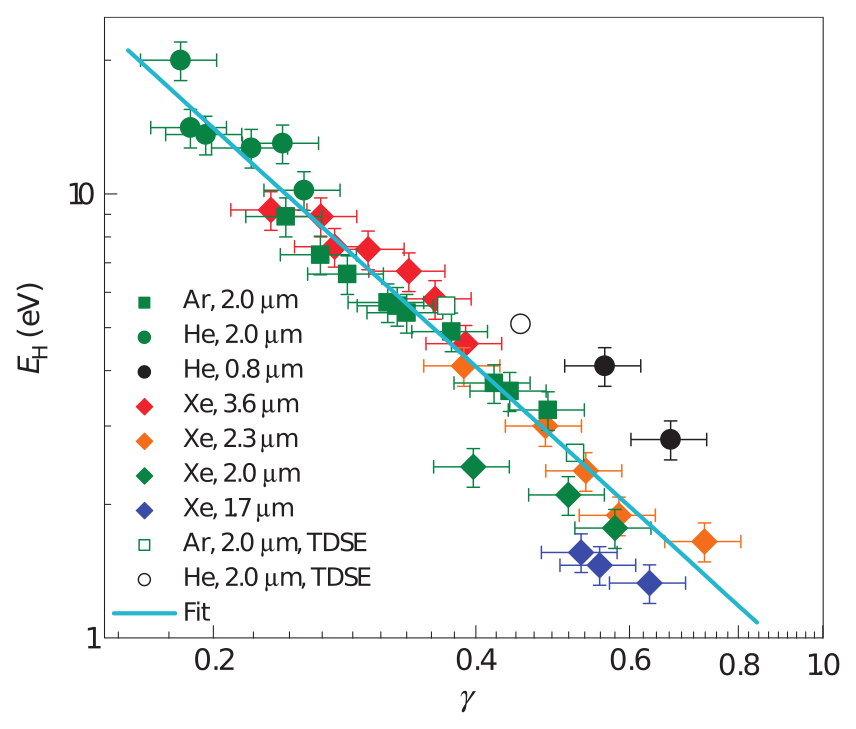
\includegraphics[scale=1]{6-LES/Figures/figure6N.png}
  \caption[
  Scaling of the upper edge energy of the LES, as measured by C.I. Blaga~et~al.
  ]{
  Scaling of the upper edge energy $E_\mathsf{H}$ of the LES structure as measured by Blaga et al.~\cite{blaga_original_LES} for multiple target species and wavelengths, over varying intensities. The scaling is essentially universal, varying with the Keldysh parameter as $E_\mathsf{H}\propto\gamma^{-2}$.
  Figure excerpted from \citer{blaga_original_LES}.
  }
\label{f6-blaga-scaling-original-figure}
\end{figure}
\copyrightfootnote{
\reffig{f6-blaga-scaling-original-figure} reprinted by permission from Macmillan Publishers Ltd: %
{\hypersetup{urlcolor=black}%
\href{http://www.nature.com/nphys}{%
\emph{Nature Phys.} \textbf{5}, p. 335 © 2009}.
}}
%% As per NPG T&Cs

Generally speaking, the LES edge is quite reliably found to scale with the Keldysh parameter as $E_\mathsf{H}\propto\gamma^{-2}$, though this can mostly be refined further to $E_\mathsf{H}\propto U_p$, with a proportionality constant close to $1/10$. This scaling essentially arises from the classical dynamics of the soft recollision within the simple man's model, and we will return to it in section \ref{sec:classical-soft-recollisions}.






%\vspace{1cm}
%\hrule
%\vspace{0.5cm}
%
%
%CTMC. \cite{CTMC1,CTMC2,CTMC3} \cite{lemell_lowenergy_2012} \cite{lemell_classicalquantum_2013}. $L{-}E$ analysis in \cite{lemell_lowenergy_2012, lemell_classicalquantum_2013}
%
%\cite{xia_near-zero-energy_2015} includes V shape \& NZES
%
%\cite{kelvich_coulomb-focusing_2015}
%
%
%%%% Exact quantum trajectories
%Full classical. Saalmann \cite{Rost_JPhysB, Rost_PRL}. %\cite{Rost_latest}.
%Becker \cite{Becker_rescattering}.
%
%%%% ISFA
%ISFA. \cite{Becker_Milosevic_quantum_orbits} \cite{Milosevic_scattering_large} \cite{Milosevic_reexamination} \cite{Becker_rescattering} 
%
%\cite{LES_Scaling} with scaling.
%
%%%% CCSFA
%Initial papers \cite{CCSFA_initial_short, CCSFA_initial_full}. Under-barrier effects \cite{TCSFA_sub_barrier}. LES via quantum orbits \cite{yan_TCSFA_caustics}.
%
%%%% Other quantum methods
%Titi \& Drake \cite{Titi_Drake_S_Matrix}. LFA \cite{Milosevic_LFA}. PSW \cite{murnane_TCSFA_tunnel_exit}. 
%
%%%% Other stuff
%
%Scaling in \cite{LES_Scaling} \cite{CTMC1} \cite{lemell_classicalquantum_2013}
%
%SMM. \cite{Becker_rescattering}. Möller's ``not Coulomb, already in SMM'' \cite{off_axis_LES}
%
%\cite{Becker_rescattering} for Coulomb bringing LES out of SMM.
%
%
%Review, \cite{agostini_ionization-review_2012}




\subsection{Theoretical explanations for near-zero energy structures}
\label{sec:NZES-theory}

As we have seen, the theoretical aspects of the LES and the VLES are relatively well understood, with a strong consensus on the fundamental roles of soft recollisions and the Coulomb field in their generation. On the other hand, the NZES is rather more recent and there is less work on the mechanisms behind it. Below, in sections~\ref{sec:ARM-soft-recollisions} and \ref{sec:classical-soft-recollisions}, we will propose a mechanism for the NZES based on an extension of the soft-recollision arguments above. At present, however, the only explanation that has been advanced relates to the role of the constant electric extraction field of the reaction microscope acting on highly excited states left over from the laser pulse~\cite{ZES_paper, Rost_latest} goes here.

It has been known for some time that if an atom is ionized by a strong laser pulse in the tunnelling regime, some fraction of the electron population taken out of the ground state is left in high-lying Rydberg states~\cite{ nubbemeyer_rydberg-creation_2008, landsman_Rydberg-creation_2015, larimian_rydberg-detection_conference_2015}, a process known as frustrated tunnelling, though relatively little is known about these states and their energy, angular momentum, and coherence characteristics. In the experiments where the NZES was observed~\cite{dura_ionization_2013, ZES_paper}, these leftover Rydberg states were also left under the action of the macroscopic electric and magnetic fields, on the order of ${\sim}\SI{1}{\volt/\centi\meter}$ and ${\sim}\SI{e-4}{\tesla}$, used by the reaction microscope to guide the electrons to the detector~\cite{moshammer_ReMi_2003}.





\begin{figure}[t]
  \centering
  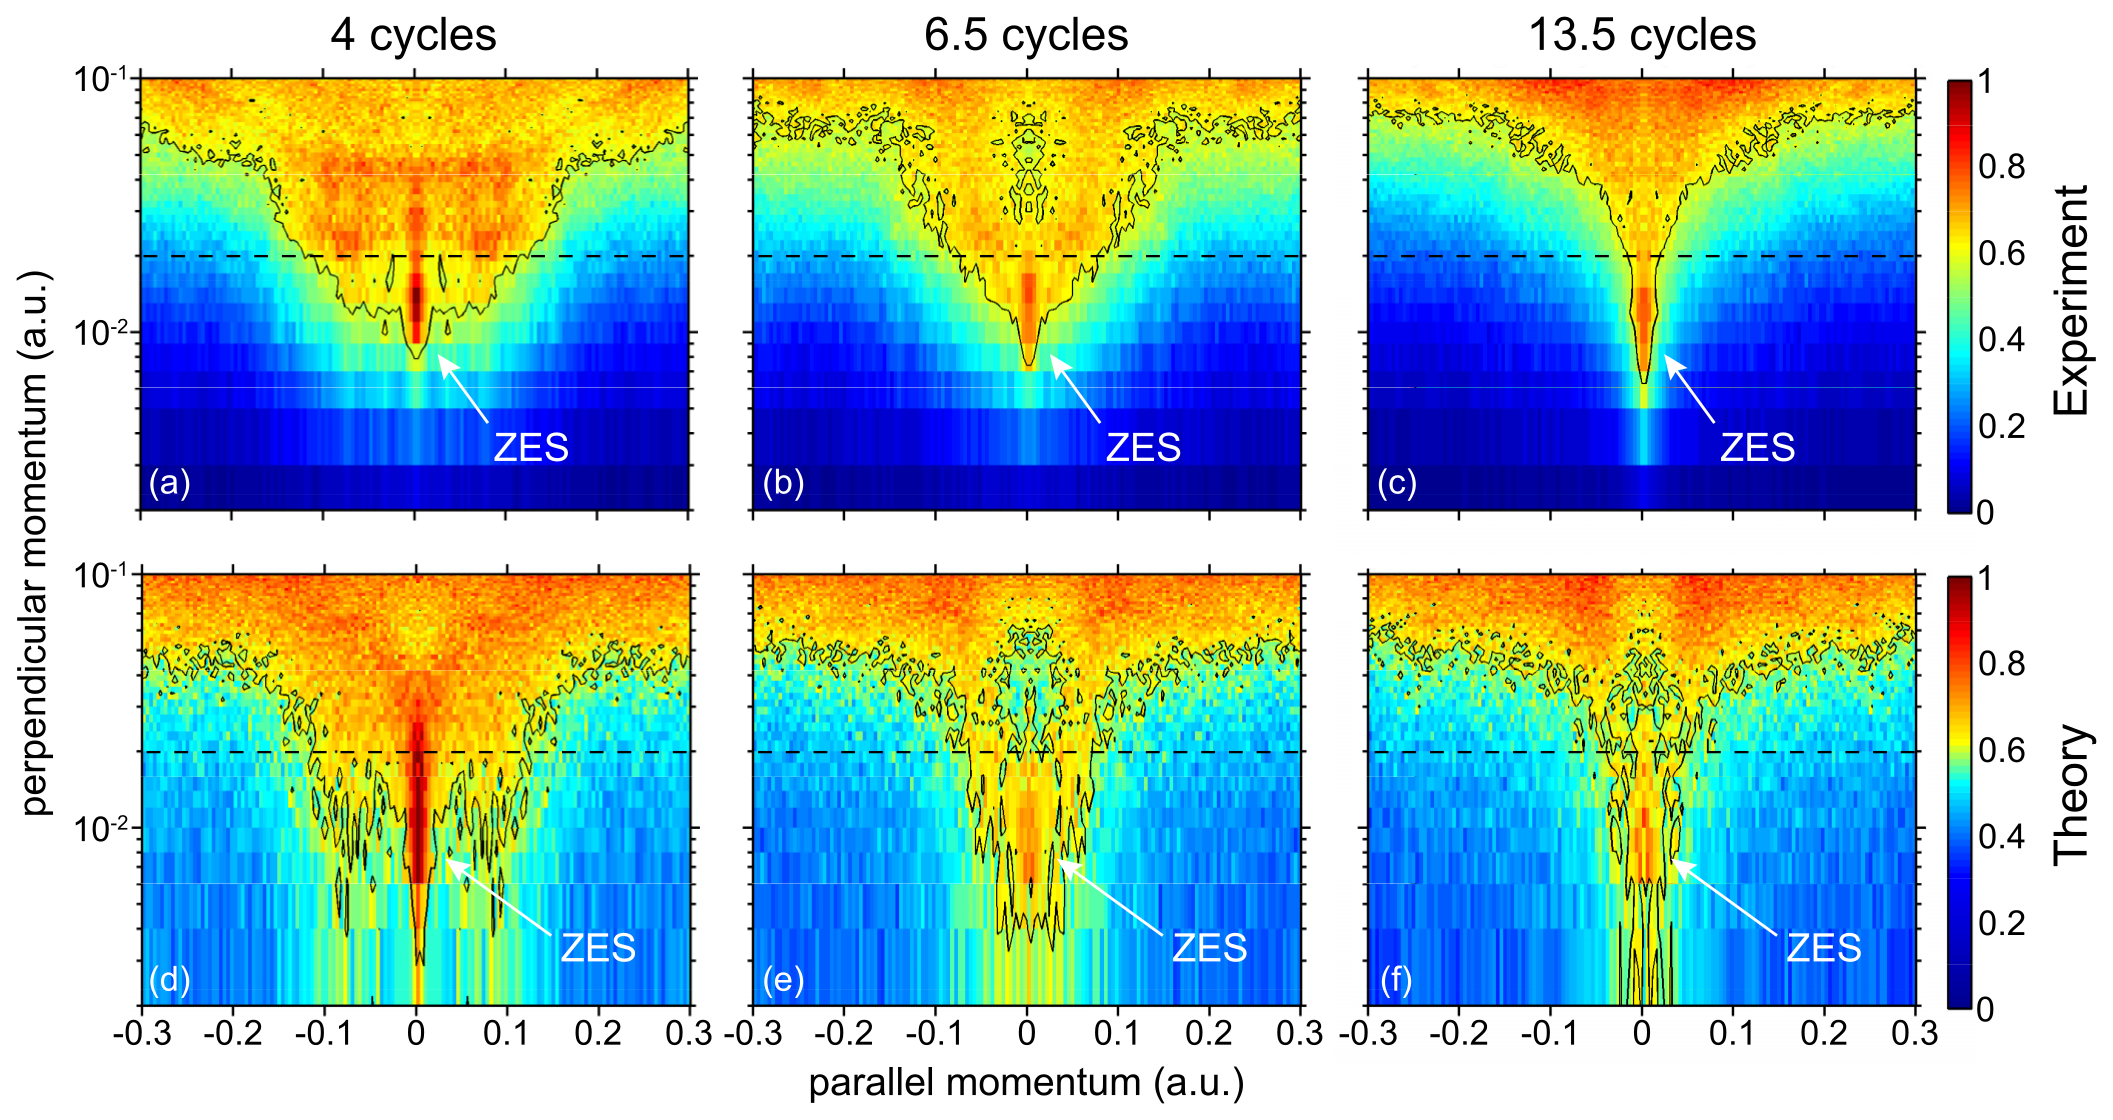
\includegraphics[width=\textwidth]{6-LES/Figures/figure6Q.png}
  \caption[
  Photoelectron momentum maps from measurements and CTMC simulations, showing a narrowing of the VLES V shape for longer pulses, together with a NZES-like structure, as observed by B. Wolter et al.
  ]{
  Ionization of argon in a $\SI{3.1}{\micro\meter}$ pulse at $\SI{9e13}{\watt/\centi\meter^2}$ at varying pulse lengths~\cite{ZES_paper}, providing a zoom to the low-energy region of \reffig{f6-wolter-original-figure-b}, and its comparison with an equivalent CTMC simulation with the extraction field accounted for. The NZES structure also appears in the CTMC simulation, which agrees with experiment on the narrowing of the VLES V shape.
  Figure excerpted from \citer{ZES_paper}.
  }
\label{f6-wolter-nzes-original-figure}
\end{figure}
\copyrightfootnote{
\reffig{f6-wolter-nzes-original-figure} reprinted with permission from B. Wolter et al., {%
\hypersetup{urlcolor=black}%
\href{http://dx.doi.org/10.1103/PhysRevA.90.063424}{%
\emph{Phys.\ Rev.\ A} \textbf{90}, 063424 (2016)}. %
©~2016 by the American Physical Society.
}
}
%% As per APS T&Cs



In principle, then, the electric extraction field, weak as it is on the atomic scale (i.e.~$\SI{1}{\volt/\centi\meter}\approx \SI{2e-10}{\au}$), can still liberate these electrons either by over-the-barrier ionization, for whatever population is left above the shallow barrier caused by the extraction field, or through tunnel ionization for states just below that. Indeed, there is some evidence that some electrons can be liberated in this way, from TDSE and CTMC simulations performed in the presence of such an extraction field~\cite{ZES_paper, Rost_latest}, though these are challenging due to the long length scales involved, and -- in the case of TDSE simulations~-- only a limited number of Rydberg states can be taken into account.



\begin{figure}[!b]
  \centering
  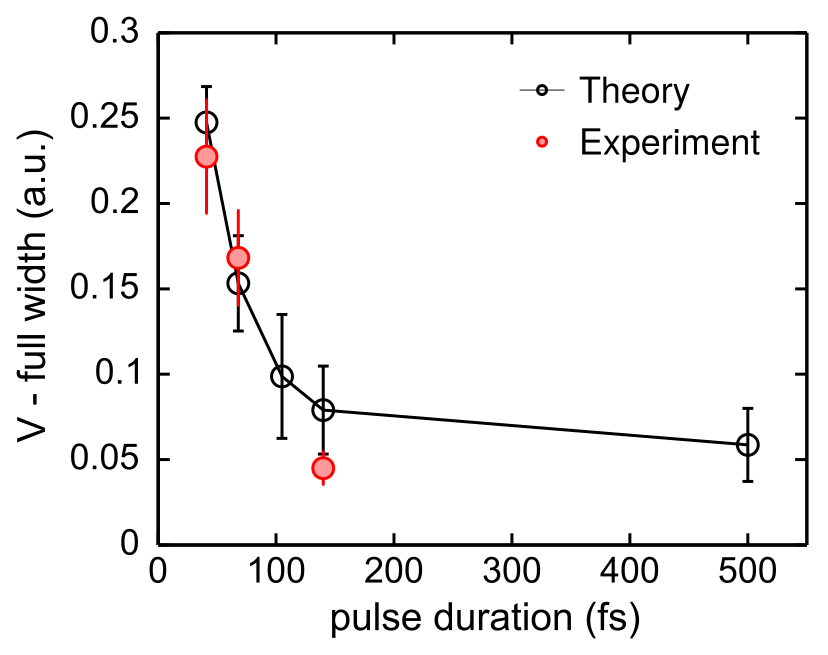
\includegraphics[scale=1]{6-LES/Figures/figure6P.png}
  \caption[
  Variation of the width of the VLES V shape with respect to the pulse length, as observed and CTMC-simulated by B. Wolter et al.
  ]{
  Variation of the width of the VLES V shape in \reffig{f6-wolter-nzes-original-figure} with respect to variations in the pulse length, showing good agreement between CTMC simulations and experiment.
  Figure excerpted from \citer{ZES_paper}.
  }
\label{f6-wolter-scaling-original-figure}
\end{figure}
\copyrightfootnote{
\reffig{f6-wolter-scaling-original-figure} reprinted with permission from B. Wolter et al., {%
\hypersetup{urlcolor=black}%
\href{http://dx.doi.org/10.1103/PhysRevA.90.063424}{%
\emph{Phys.\ Rev.\ A} \textbf{90}, 063424 (2016)}. %
©~2016 by the American Physical Society.
}
}
%% As per APS T&Cs


Nevertheless, the structure does appear in CTMC simulations with the extraction field, as shown in \reffig{f6-wolter-nzes-original-figure}, and it shows some agreement with experiment. Moreover, CTMC calculations agree with experiment on the width of the VLES V shape as the length of the laser pulse changes, with the scaling shown in \reffig{f6-wolter-scaling-original-figure}.



In addition to this, the extraction-field mechanism requires that the characteristics of the NZES peak change as the strength of the extraction field changes. This is a hard prediction to explore experimentally, because the extraction field is also a crucial variable both in how many electrons are detected as well as in fixing the final resolution of the detector (i.e. the level of zoom into the photoelectron momentum distribution), so variations there have a strong effect on the rest of the experiment, but there are indeed some hints of variation in the width of the structure in experiment, as shown in \reffig{f6-diesen-scaling-original-figure}. 

Moreover, there is also some agreement between the observed experimental variations and a simplified semiclassical theory which considers classical electrons, uniformly distributed in Rydberg states just below the ionization threshold, in a single rescaled Coulomb potential plus the extraction field~\cite{Rost_latest}.

On the other hand, the extraction-field mechanism would also require the yield of the structure -- the number of electrons in the NZES -- to change with the extraction field, since if the pulse parameters don't vary then the Rydberg population will not change appreciably, and a stronger extraction field will lower the shallow barrier and thereby liberate a larger population of electrons. (Even further, the Rydberg population is expected to be roughly uniformly distributed over energy just below threshold, so the NZES yield should scale roughly linearly with the extraction field over its $\sim$tenfold variation in \citer{Rost_latest}.) However, this is rather difficult to test experimentally, since changing the extraction field has a strong effect on the entire detection, and there is at present no evidence for this dependence, which represents the clearest way forward in validating this mechanism as a contributor to the NZES.


\begin{figure}[t]
  \centering
  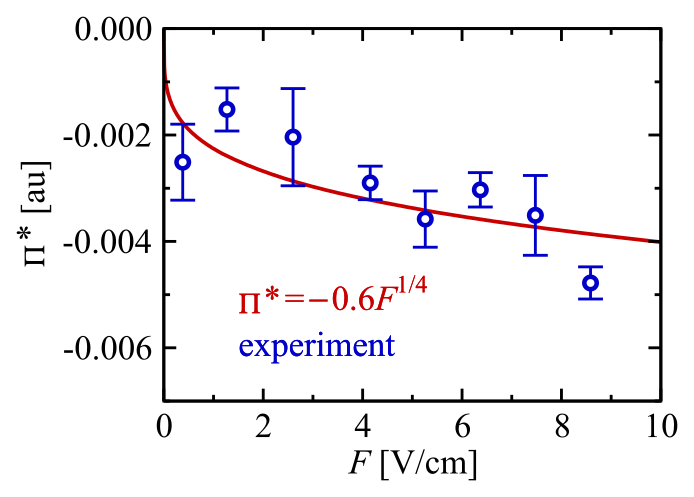
\includegraphics[scale=1.15]{6-LES/Figures/figure6O.png}
  \caption[
  Measured momentum width of the NZES, compared with predictions from extraction-field theory, as observed by E. Diesen et al.
  ]{
  Momentum width $\Pi^*$ of the NZES in ionization of $\mathrm{N_2}$ in a $\SI{780}{\nano\meter}$ pulse, subsequently ionized by extraction fields of different strengths, showing some variation in the width of the feature with the extraction field strength. The red curve shows the predicted width of extraction from a rescaled Coulomb potential.
  Figure excerpted from~\citer{Rost_latest}.
  }
\label{f6-diesen-scaling-original-figure}
\end{figure}
\copyrightfootnote{
\reffig{f6-diesen-scaling-original-figure} reprinted with permission from E. Diesen et al., {%
\hypersetup{urlcolor=black}%
\href{http://dx.doi.org/10.1103/PhysRevLett.116.143006}{%
\emph{Phys.\ Rev.\ Lett.} \textbf{116}, 143006 (2016)}. %
©~2016 by the American Physical Society.
}
}
%% As per APS T&Cs




\section[Soft recollisions in Analytical R-Matrix theory]{Soft recollisions in Analytical $R$-Matrix theory}
\label{sec:ARM-soft-recollisions}

Having seen the current understanding of the LES in the literature, we now turn to what our ARM theory of photoionization can tell us about soft recollisions and their role in photoelectron spectra. 

As we have seen, the ARM formalism works with a different set of trajectories to the ones mentioned above, since it does not use the full Coulomb-laser trajectory used by full classical CTMC theories and by the semiclassical CCSFA, nor does it use the real-valued simple-man's trajectories with only the laser driving as in \citer{ off_axis_LES}. In those real-time theories, the soft recollision shows up topologically as a topological change in the trajectory, as shown in \reffig{f5-classical-tca-on-axis}, and the number of extrema of $\rcl(t)^2$ along the path: from a single inwards turning point, to an outwards turning point flanked by two closest-approach times, as shown in \reffig{f5-sample-trajectories-a}.

The ARM trajectories, on the other hand, are different, because the trajectory path through the complex time plane is no longer constrained to lie on the real axis, which means that the closest-approach solutions are not lost -- they simply go off into the complex plane, where they can still be reached by the integration path over the complex time plane if there is a strong enough reason (such as avoiding Coulomb branch cuts) to do so. The last time we considered the soft recollisions in this context, then, was as a complex interaction between pairs of branch cuts, depicted in \reffig{f5-branch-cut-topology-change}, at which two pairs meet and recombine, changing the branch cut topology that the integration path needs to navigate.


Moreover, although we showed in \reffig{f5-branch-cut-topology-change} a single example at a return time of $\omega t\approx 2\pi$, this behaviour reoccurs every half period thereafter, as is clear from the quantum $\tca$ surface we saw in \reffig{f5-quantum-tca-surface}. Here, for clarity, we revisit \reffig{f5-branch-cut-topology-change}, showing in \reffig{f6-branch-topology-revisited} the change in the branch cut topology of $\sqrt{\rl(t)^2}$ for the first soft recollision, at $\omega t\approx 2\pi$ and a very low momentum, and the second one at $\omega t\approx 3\pi$ and a slightly higher momentum.


\captionsetup[figure]{position=top}

\begin{figure}[htb]
\centering
  \begin{tabular}{cc}
  $\qquad p_z=\figurefiveKppl{}F/\omega$   &    $p_z=\figurefiveKpph{}F/\omega$  
  \\  \hline  \vspace{-2mm} \\
  \subfloat[$\sqrt{\rl(t)^2}$\hspace{-6pt}$\,$]{
    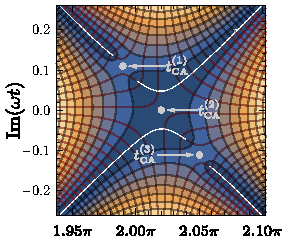
\includegraphics[scale=\figurefiveKscale]{6-LES/Figures/figure6-2Aa.pdf}
    \label{f6-branch-cut-topology-open-one}
  }
  & \hspace{-6mm}
  \subfloat[$\sqrt{\rl(t)^2}$ \hspace{25pt}$\,$]{
    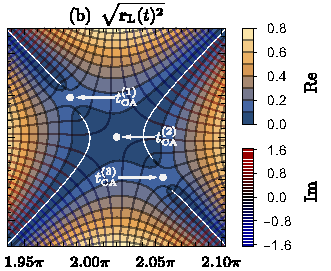
\includegraphics[scale=\figurefiveKscale]{6-LES/Figures/figure6-2Ab.pdf}
    \label{f6-branch-cut-topology-closed-one}
  }
  \\[10mm]
  $\qquad p_z=\figuresixtwoAppltwo{}F/\omega$   &    $p_z=\figuresixtwoApphtwo{}F/\omega$   
  \\  \hline  \vspace{-2mm} \\
  \subfloat[$\sqrt{\rl(t)^2}$\hspace{-6pt}$\,$]{
    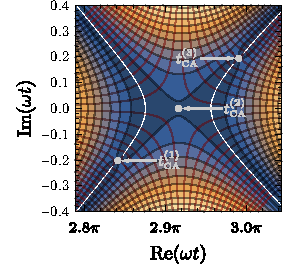
\includegraphics[scale=\figurefiveKscale]{6-LES/Figures/figure6-2Ac.pdf}
    \label{f6-branch-cut-topology-open-two}
  }
  & \hspace{-6mm}
  \subfloat[$\sqrt{\rl(t)^2}$ \hspace{25pt}$\,$]{
    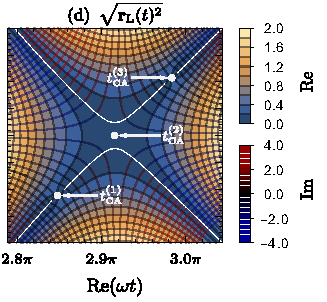
\includegraphics[scale=\figurefiveKscale]{6-LES/Figures/figure6-2Ad.pdf}
    \label{f6-branch-cut-topology-closed-two}
  }
  \end{tabular}
  \caption[
  Change in the branch cut topology for the first two soft recollisions
  ]{
  Change in the branch cut topology, as in  \reffig{f5-branch-cut-topology-change}, for the first two soft recollisions. Note that the order of the transition (open to closed, and vice versa) is reversed with respect to increasing $p_z$.
}
\label{f6-branch-topology-revisited}
\end{figure}

\captionsetup[figure]{position=auto}







As we saw in chapter~\ref{chap:quantum-orbits}, these soft recollisions are the hardest point for the branch cut navigation, since they provide the closest gates with a very sensitive dependence on the problem's parameters. This is emphasized by the very small momentum changes between the left and right columns of \reffig{f6-branch-topology-revisited}, which mark the change in topology, and therefore the switch in the choice of closest-approach times the integration path needs to go through.

In addition to this, however, the soft recollisions also have a strong effect on the ionization amplitude, because these drastic changes in the integrand occur precisely when it is at its largest. Thus, choosing the wrong contour in this region accounts for the largest contributions to the integrand, with a correspondingly large effect on the integral, so correctly navigating the cuts here is even more crucial. 

More surprisingly, however, once the contour is forced to pass through the `gate' $\tca$s, for $p_z$ just on the `closed-gate' topology side of $\pzsr$, the contributions of those saddles have the effect of suppressing the ionization amplitude there.

To see how this comes about, consider the integral $\int U(\rcl(t))\d t$ for the configuration of \reffig{f6-branch-cut-topology-open-one}. Here $\sqrt{\rcl(t)^2}$ has a minimum at the central saddle point, $\tcasup{\,(2)}$, and this translates into a maximum of $1/\sqrt{\rcl(t)^2}$ which dominates the integral. At this point, the approach distance 
\begin{equation}
r_\ast=\sqrt{\rcl(\tcasup{\,(2)})^2}
\end{equation}
is dominated by a modest and positive imaginary part. This means that 
\begin{equation}
U_\ast=-1/r_\ast
\end{equation}
is large and (positive) imaginary, and therefore the correction factor $e^{-i\int U\d t}$ has a large amplitude.

On the other hand, in the configuration of \reffig{f6-branch-cut-topology-closed-one} the integral is dominated by the `gate' closest-approach times, for  which
\begin{equation}
r_\ast'=\sqrt{\rcl(\tcasup{\,(1)})^2}\approx\sqrt{\rcl(\tcasup{\,(1)})^2}
\end{equation} 
is mostly real and much smaller than $r_\ast$. The corresponding potential $U_\ast'=-1/r_\ast'$ is then large, real and negative, and $-iU_\ast'$ is along $+i$. However, here the line element $\d t$ must slope upwards with a positive imaginary part to emphasize the contribution of the saddle point, and this then gives $-i\int U(\rcl(t))\d t$ a large and negative real part. This, in turn, suppresses the amplitude of the correction factor $e^{-i\int U\d t}$. 




This effect is then visible in the photoelectron spectrum as a large peak just below the soft recollision, followed by a deep, narrow dip, which we show in \reffig{f6-po-pp-spectrum}. In an experimental setting, the dip will almost certainly get washed out by nearby contributions unless specific steps are taken to prevent this, but the peak will remain. (In addition, this effect mirrors the redistribution of population seen in classical-trajectory-based approaches, where the peaks caused by dynamical focusing represent trajectories taken from other asymptotic momenta, whose amplitude is therefore reduced.)


\begin{figure}[htb]
  \centering
  \begin{tabular}{c}
    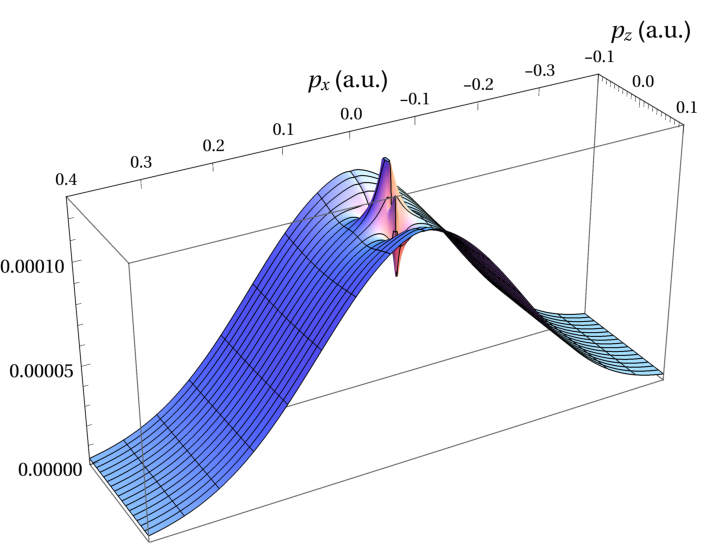
\includegraphics[width=0.7\columnwidth]{6-LES/Figures/figure6-2B.pdf}
  \end{tabular}
  \caption[
  ARM photoelectron spectra showing Near-Zero Energy Structures
  ]{
  Emergence of the Near-Zero Energy Structures within the Analytical $R$-Matrix theory: incoherent addition of the sub-cycle ionization yields for two adjacent half-cycles, $\tfrac12\big(\left|a(p_x,0,p_z)\right|^2+\left|a(p_x,0,-p_z)\right|^2\big)$, as predicted by the ARM amplitude.
  We ignore the shape factor $R(\vbp)$, and consider for the ionization of unaligned molecular nitrogen by a $\SI{\figuresixtwoBwavelength}{\micro\meter}$ field at $\SI{e14}{\watt/\centi\meter^2}$, with $\gamma=\figuresixtwoBgamma$, as per the parameters of \citer{ pullen_kinematically_2014} whose experimental data is shown in Figs.~\ref{f6-pullen-original-full-spectrum} and \ref{f6-pullen-original-transverse-spectrum}. The Coulomb-correction has been integrated over 2.75 laser periods. 
  }
  \label{f6-po-pp-spectrum}
\end{figure}


Here the peak in \reffig{f6-po-pp-spectrum} should be compared with the experimental transverse spectra we showed earlier in \reffig{f6-pullen-original-transverse-spectrum}, which also displayed a sharp spike rising out of a gaussian background for very small longitudinal momentum. Here the spike is not as sharp (it is shown in linear scale instead of logarithmic scale) but given the approximations in ARM theory it is only expected to produce qualitative agreement, which is indeed very striking. 

For this specific case, the momentum scales involved are really very low: here there are two closely spaced transitions at $\pzsr{}= \SI{ \figuresixtwoBfirstpztransition }{\au}$ and $\pzsr{}=\SI{\figuresixtwoBthirdpztransition}{\au}$ (with some interplay between them showing up), and this is roughly at the state of the art of momentum resolution, $\Delta p\sim\SI{0.02}{\au}$, claimed by recent experiments~\cite{ pullen_kinematically_2014, Wolter_PRX}; in terms of energy, it corresponds to a photoelectron energy of about $\SI{8}{\milli\electronvolt}$. Thus, the ARM peak has a finite width, but this is too small to be resolved at present and structures at this range would show up simply as consistent with zero.


The peak in \reffig{f6-po-pp-spectrum} is clearly similar to the NZES structure, as experimentally observed, so it calls for further exploration. Since it is directly associated with the soft recollisions of the previous chapter, we have a clear indication of the possible mechanism for the structure, and we will examine the connection further in the next section.




Finally, it is worth noting that a more recent CCSFA analysis of ATI~\cite{ keil_branch-cuts_2016}, using a complex tunnel exit as in ARM theory (and thereby restricted to only a laser-driven trajectory), and relying on the branch-cut navigation algorithm we developed in chapter~\ref{chap:LES-NZES}, confirms our findings of LES peaks in this energy region.









\section{Classical soft-recollision trajectories}
\label{sec:classical-soft-recollisions}
We have seen, then, that our ARM theory of photoionization predicts a sharp peak at very low electron energies, and we know the class of trajectories -- soft recollisions -- that underpin it. Moreover, we have been forced by our integration-path selection algorithm to grapple with soft recollisions every half cycle, with the complex topological changes depicted in \reffig{f6-branch-topology-revisited} occurring at $\omega t\approx 2\pi,3\pi,4\pi,\ldots$, giving a distinct series of trajectories and therefore a distinct series of LES structures, some of which we have already covered.

However, these trajectories come in two distinct flavours, as depicted in \reffig{f6-trajectories-at-transitions}: one class (shown in dashed red) with the soft recollision on a `backwards' turning point, at $\omega t\approx 3\pi, 5\pi, 7\pi, \ldots$, and a second class with the soft recollision on the `forwards' turning points, at $\omega t\approx 2\pi, 4\pi, 6\pi, \ldots$, shown in solid blue.

\begin{figure}[ht]
  \centering
  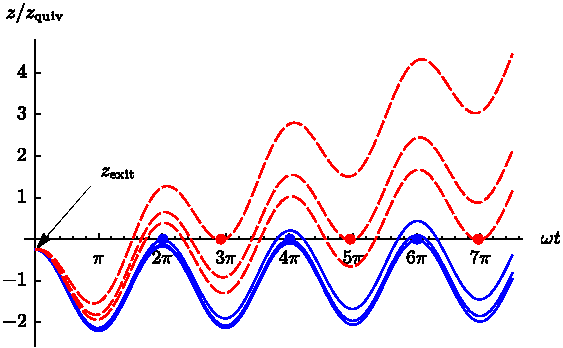
\includegraphics[width=0.6\columnwidth]{6-LES/Figures/figure6-2D.pdf}
  \caption[
  Trajectories with soft recollisions, both on the backwards swing and the forwards turning point
  ]{
  Trajectories with soft recollisions after tunnel ionization, for a Keldysh parameter of  $\gamma=\figuresixtwoDgamma$.}
  \label{f6-trajectories-at-transitions}
\end{figure}

The first class we have already met, in \reffig{f6-rost-soft-recollisions} and first described in Refs.~\citealp{Rost_PRL} and \citealp{Rost_JPhysB}, but the second class has received very little attention in the literature, essentially because most analyses of the soft recollisions as a marker for the LES peaks have used models where the electron trajectory starts at the origin~\cite{Becker_rescattering}. At first blush, ignoring the tunnel exit $\zexit\sim I_p/F$ is relatively safe, since at the wavelengths of interest the quiver amplitude $\zquiv=F/\omega^2$ is much larger, as shown in \reffig{f6-trajectories-at-transitions}. However, for the second class of trajectories, if one ignores the tunnel exit then the whole series collapses into a single trajectory at zero momentum, thereby washing out all the dynamics. However, any reasonable theory of optical tunnelling should place the electrons at the tunnel exit, and doing this unfolds the second series into distinct trajectories.

Moreover, it is quite possible to describe the trajectories shown in \reffig{f6-rost-soft-recollisions} within the quasi-classical formalism that simply looks for real-valued trajectories on real times, and this will help us better understand their characteristics. We retake, then the classical trajectories
\begin{equation}
\rcl(t) = \Re\left(\int_{\ts}^{t} \left[ \vbp+\vba(\tau) \right] \: \d\tau\right)
\backtag{e5-classical-trajectory}
\end{equation}
from section~\ref{sec:classical-tcas}, as our classical trajectories. Within these trajectories, we define the soft recollisions as those real times $\tr$ for which both the velocity and the real part of the trajectory vanish, so that
\begin{subequations}
\label{e6-symbolic-system}
\begin{empheq}[left=\empheqlbrace]{align}
\zcl(\tr)&=\Re\left[ \int_\ts^{\tr} \left(p_z+A(\tau)\right)\d\tau\right]=0 \\
v_z(\tr)&=p_z+A(\tr)=0.
\end{empheq}
\end{subequations}


Putting in explicit values for the vector potential and its integral, this can then be re-expressed as
\begin{subequations}
\label{e6-spelled-out-system}
\begin{empheq}[left=\empheqlbrace]{align}
\zexit+p_z(\tr-\tn)+\frac{F}{\omega^2}\left(\cos(\omega\tr)-\cos(\omega\tn)\right)  &=0 \\
p_z-\frac F\omega \sin(\omega\tr)  &=0,
\end{empheq}
\end{subequations}
where
\begin{align}
\zexit
&=
\Re\left[ \int_\ts^\tn \left(p+A(\tau)\right)\d\tau\right]
%\nonumber\\ &
=
\frac{F}{\omega^2}\cos(\omega\tn) \left(1- \cosh(\omega\tauT)\right)
\end{align}
models the tunnel exit, and reduces to the standard $\zexit\approx -I_p/F$ in the tunnelling limit where  $\gamma\ll 1$.

This system of equations, \eqref{e6-spelled-out-system}, can be solved numerically rather easily, but it is more instructive to consider its linearized version with respect to $p_z$, since all the soft recollisions happen at small energies with respect to $U_p$. To do this, we express the starting time as
\begin{align}
\tn+i\tauT=\ts
& = \frac1\omega  \arcsin\left(\frac{\omega}{F}(p_z+i\kappa)\right)
%\nonumber\\& 
\approx  
\frac{ p_z}{F}\frac{1}{\sqrt{1+\gamma^2}} + \frac{i}{\omega}\arcsinh\left(\gamma\right),
\end{align}
where $\gamma=\omega\kappa/F$ is the Keldysh parameter as usual, so that $\zexit \approx - \frac{F}{\omega^2}\left(\sqrt{1+\gamma^2}-1\right)$. The linearized system now reads
\begin{subequations}
\begin{empheq}[left=\empheqlbrace]{align}
p_z\tr+\frac{F}{\omega^2}\left(\cos(\omega\tr)-\sqrt{1+\gamma^2}\right)  &=0 \\
p_z-\frac F\omega \sin(\omega\tr)  &=0,
\label{e6-pz-to-tr-eqn}
\end{empheq}
\end{subequations}
and to obtain a solution we must linearize $\tr$ with respect to $p_z$. It is clear from \reffig{f6-trajectories-at-transitions}, and from the numerical solutions of \eqref{e6-spelled-out-system}, that the solutions occur close to each $(n+1)\pi$ for $n=1,2,3,\ldots$, so it is justified to write
\begin{equation}
\omega \tr= (n+1)\pi+\omega \,\delta\tr,
\end{equation}
where we expect $\delta\tr$ to be small. 


Putting this in we obtain from \eqref{e6-pz-to-tr-eqn} that $\delta\tr\approx(-1)^{n+1}p_z/F$ and $\cos(\omega\tr) \approx(-1)^{n+1}$, and this gives in turn the drift momentum of the successive soft-recolliding trajectories as 
\begin{equation}
\pzsr \approx \frac F\omega \frac{\sqrt{1+\gamma^2}+(-1)^n}{(n+1)\pi}.
\label{e6-linearized-momenta}
\end{equation}
These are shown in \reffig{f6-soft-recollision-scaling}  , and they are generally a good approximation to the exact solutions of \eqref{e6-spelled-out-system}, shown dotted.


\begin{figure}[htb]
  \centering
  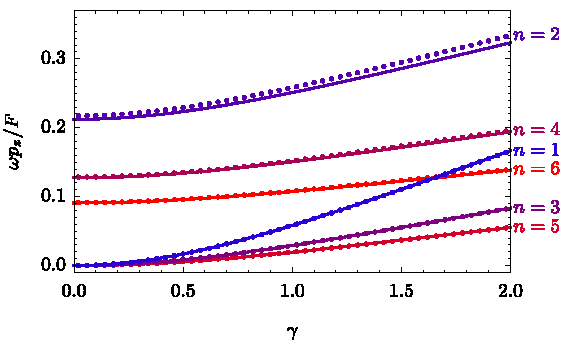
\includegraphics[scale=1]{6-LES/Figures/figure6-2E.pdf}
  \caption[
  Scaling of the soft-recollision momentum as a function of the Keldysh parameter
  ]{
  Scaling of the normalized soft-recollision momentum $\omega p_z/F$ as a function of the Keldysh parameter $\gamma$ for the first six soft-recollision trajectories. Dots show the exact solutions of \eqref{e6-symbolic-system} and lines show the linearized result \eqref{e6-linearized-momenta}.
  }
  \label{f6-soft-recollision-scaling}  
\end{figure}

Here it is quite clear that the trajectories with even $n$ -- our new series, shown solid blue in \reffig{f6-trajectories-at-transitions} -- will scale very differently than the previously known series, which has odd $n$ and was shown in dotted red in \reffig{f6-trajectories-at-transitions}. This scaling, in fact, holds the key to the physical differences between the two classes of trajectories, so it is worth spending some time teasing out its roots and implications.

\begin{itemize}

\item Starting with the even-$n$ trajectories, we can further simplify the momentum to 
\begin{equation}
\pzsr \approx \frac F\omega \frac{\sqrt{1+\gamma^2}+1}{(n+1)\pi},
\end{equation}
which for low $\gamma$ simplifies to
\begin{equation}
\pzsr 
\approx \frac F\omega \frac{2+\frac12 \gamma^2}{(n+1)\pi}
=\frac F\omega \frac{2}{(n+1)\pi}
\approx 2\,\frac{F}{\omega^2} \frac{\omega}{(n+1)\pi}.
\label{e6-even-n-scaling}
\end{equation}
This last form holds most of the physical content for the scaling, because it separates into twice the quiver radius, $2\zquiv=2F/\omega^2$, split over the time between the ionization and the recollision, $(n+1)\pi/\omega$, and this is clearly the distance that the oscillation centroid of the even-$n$ trajectories needs to cover in \reffig{f6-trajectories-at-transitions} for the backwards turning points to pass through the origin.

Moreover, this scaling now gives us a direct line on the behaviour of the LES, because it can be directly translated into an estimate of the signature kinetic energy of the structure,
\begin{equation}
\frac12 \left(\pzsr\right)^2 
\approx \frac{F^2}{\omega^2}\frac{2}{(n+1)^2\pi^2}
=\frac{8}{(n+1)^2\pi^2} U_p,
\end{equation}
where the $\pzsr\sim F/\omega$ momentum scaling translates directly into an energy that scales directly with the ponderomotive potential $U_p$. Further, the numerical constant evaluates to roughly $\frac{1}{10}$. The linearity with respect to $U_p$, together with the numerical constant, matches the known scaling of the LES, as discussed at the end of section~\ref{sec:LES-theory}.

\item Turning to the odd-$n$ trajectories, the $\cos(\omega\tr)\approx (-1)^n$ factor is now odd -- we are on a forwards swing of the orbit -- and this means that the momentum will behave differently, since now
\begin{equation}
\pzsr 
\approx \frac F\omega \frac{\sqrt{1+\gamma^2}-1}{(n+1)\pi}
\approx \frac F\omega \frac{\gamma^2}{2(n+1)\pi}
\approx \frac{\gamma\kappa}{2(n+1)\pi}
\approx \frac{\omega}{F} \frac{\kappa^2/2}{(n+1)\pi}.
\label{e6-pzsr-odd-n-full}
\end{equation}
This scaling is somewhat more complicated, and it is in fact one of the central results of this work; simple as it is, it seems to have avoided description so far.

To begin with, the form $\pzsr\sim \gamma \kappa$, obtained by trading in one factor of $\gamma=\kappa\omega/F$, implies that the high-energy edge of this NZES structure will scale as $\gamma^2$ for a fixed target species, and this marks a straight departure from the LES scaling, which goes~as~$\gamma^{-2}$.

Finally, the last form of the soft-recollision momentum $\pzsr$ in \eqref{e6-pzsr-odd-n-full} tells the rest of the tale, since it can be cleanly reorganized as 
\begin{equation}
\pzsr 
\approx \frac{\zexit}{\Delta t}
= \frac{I_p/F}{(n+1)\pi/\omega}
\propto \frac{I_p\omega}{F},
\label{e6-pzsr-odd-n-summary}
\end{equation}
giving the distance to be covered -- the tunnel width, $\zexit\approx I_p/F$, over the time $\Delta t=(n+1)\pi/\omega$ between ionization and recollision.

\end{itemize}


This last form also marks in a clean way the real difference in scalings between the usual even-$n$ trajectories and our odd-$n$ ones, because when translated into energy it reads
\begin{equation}
\frac12\left(\pzsr\right)^2 
\sim \frac{I_p^2}{U_p}
\sim I_p\gamma^2,
\label{e6-odd-n-energy-scaling}
\end{equation}
that is, for a fixed target species the high-energy edge of this structure should be expected to scale \textit{inversely} with respect to the ponderomotive potential $U_p$, which is completely opposite to the usual behaviour of the LES series.

In addition to this, the energy scaling in \eqref{e6-odd-n-energy-scaling} is also immensely valuable in that it directly suggests the experimental avenues that will help resolve the contribution of our odd-$n$ trajectory series to the observed NZES experimental feature. As we argued earlier, the NZES has so far only been observed to be at energies consistent with zero to the experimental accuracy, and any tools that can help lift this feature to higher energies where the detectors -- already at their state-of-the-art resolution -- can resolve them better will be a valuable avenue for exploration. 





%
%\begin{figure}[ht]
%  \centering
%  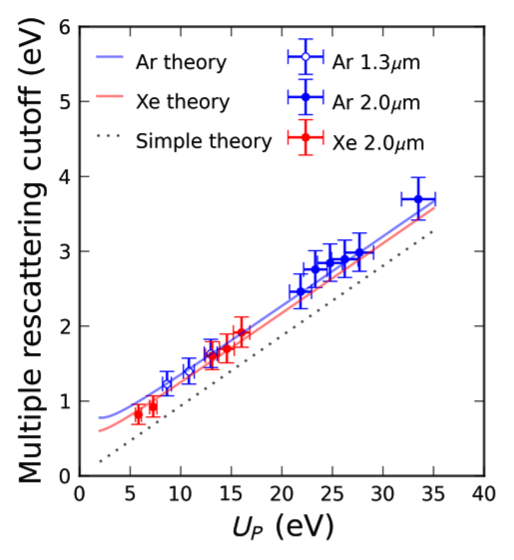
\includegraphics[scale=1.2]{6-LES/Figures/figure6R.png}
%  \caption[
%  Experimental scaling of the LES width, as observed by D.D. Hickstein et al., showing departures from the naive theory caused by the tunnel width
%  ]{
%  Scaling of the LES width for ionization of argon and xenon in $\SI{1.3}{\micro\meter}$ and $\SI{2}{\micro\meter}$ fields at varying intensity, with respect to the ponderomotive energy of the field. The naive scaling as per~\eqref{e6-even-n-scaling} is shown dashed, while the solid lines denote a semiclassical tunnelling theory with the tunnel exit included, as in~\eqref{e6-even-n-scaling-with-zexit}.
%  Figure excerpted from \citer{murnane_TCSFA_tunnel_exit}.
%  }
%\label{f6-hickstein-scaling-original-figure}
%\end{figure}
%\copyrightfootnote{
%\reffig{f6-hickstein-scaling-original-figure} reprinted with permission from D.D. Hickstein et al., {%
%\hypersetup{urlcolor=black}%
%\href{http://dx.doi.org/10.1103/PhysRevLett.109.073004}{%
%\emph{Phys.\ Rev.\ Lett.} \textbf{109}, 073004 (2012)}. %
%©~2012 by the American Physical Society.
%}
%}
%%% As per APS T&Cs


In particular, for the tunnelling mechanism to hold well we require that the Keldysh parameter $\gamma$ be small, which therefore means that if we want the energy in \eqref{e6-odd-n-energy-scaling} to be large this can only be done by going to harder targets with a higher ionization potential; this would ideally be helium, or if possible the helium ion $\mathrm{He^+}$, either as an ionic beam or prepared locally via sequential ionization or a separate pre-ionizing pulse. (In any case, the requirement of a high $I_p$ is consistent with the weak NZES structure observed in xenon~\cite{Wolter_PRX}, which we reproduced in \reffig{f6-wolter-prx-original-figure}.) The scaling in \eqref{e6-odd-n-energy-scaling} is certainly unfavourable, but it points the way to experiments which should be able to resolve whether this mechanism contributes or not. 




As a separate observation, it is interesting to note that the $\gamma^2$ term that is crucial to the scaling of the odd-$n$ trajectories is in fact also present for the even-$n$ scaling, which can be refined to the form

\begin{equation}
\pzsr 
\approx \frac F\omega \frac{2+\frac12 \gamma^2}{(n+1)\pi}
= \left(2\frac{F}{\omega^2}+\frac{I_p}{F}\right) \frac{\omega}{(n+1)\pi}
= \frac{2\zquiv + \zexit}{(n+1)\pi/\omega},
\label{e6-even-n-scaling-with-zexit}
\end{equation}
which cleanly expresses the fact, shown in \reffig{f6-trajectories-at-transitions}, that the odd-$n$ trajectories also need to traverse the tunnel exit to make their soft-recollision date with the ion; here the $\zexit$ contribution is small but it is still present. In fact, this difference in the scaling properties of the LES energy has already been observed~\cite{murnane_TCSFA_tunnel_exit}, and we reproduce the result in \reffig{f6-hickstein-scaling-original-figure}.





\begin{figure}[ht]
  \centering
  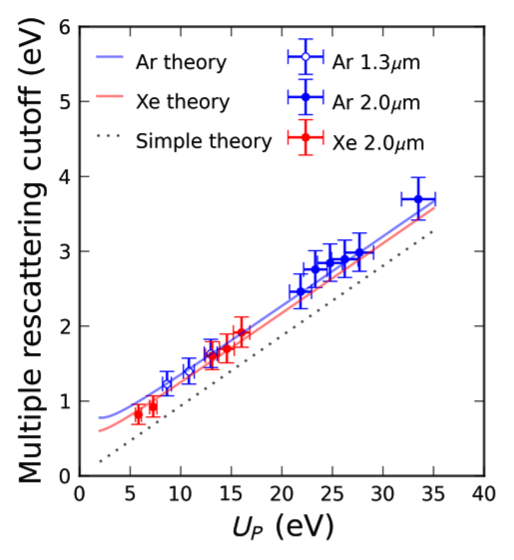
\includegraphics[scale=1.2]{6-LES/Figures/figure6R.png}
  \caption[
  Experimental scaling of the LES width, as observed by D.D. Hickstein et al., showing departures from the naive theory caused by the tunnel width
  ]{
  Scaling of the LES width for ionization of argon and xenon in $\SI{1.3}{\micro\meter}$ and $\SI{2}{\micro\meter}$ fields at varying intensity, with respect to the ponderomotive energy of the field. The naive scaling as per~\eqref{e6-even-n-scaling} is shown dashed, while the solid lines denote a semiclassical tunnelling theory with the tunnel exit included, as in~\eqref{e6-even-n-scaling-with-zexit}.
  Figure excerpted from \citer{murnane_TCSFA_tunnel_exit}.
  }
\label{f6-hickstein-scaling-original-figure}
\end{figure}
\copyrightfootnote{
\reffig{f6-hickstein-scaling-original-figure} reprinted with permission from D.D. Hickstein et al., {%
\hypersetup{urlcolor=black}%
\href{http://dx.doi.org/10.1103/PhysRevLett.109.073004}{%
\emph{Phys.\ Rev.\ Lett.} \textbf{109}, 073004 (2012)}. %
©~2012 by the American Physical Society.
}
}
%% As per APS T&Cs




For the odd-$n$ series, adding in the tunnel exit represents a small correction to the main result driven by the quiver radius, and this correction is mirrored by similar corrections for the cutoff position in high-harmonic generation \cite{LewensteinHHG} and in high-order above-threshold ionization \cite{ HATI_quantum_correction, HATI_quantum_correction_2, HATI_quantum_correction_3}, so this comes about as yet another example of fairly standard tunnelling theory. For our even-$n$ series of trajectories, on the other hand, this correction is applied on top of a zero result, so it becomes the driving term for the scaling dynamics of this series of trajectories.




\newcommand{\figuresixtwoCpomult}{1.5} 
\newcommand{\figuresixtwoCfield}{0.05} 
\newcommand{\figuresixtwoCkappa}{1.07}
\begin{figure}[hbt]
  \centering
  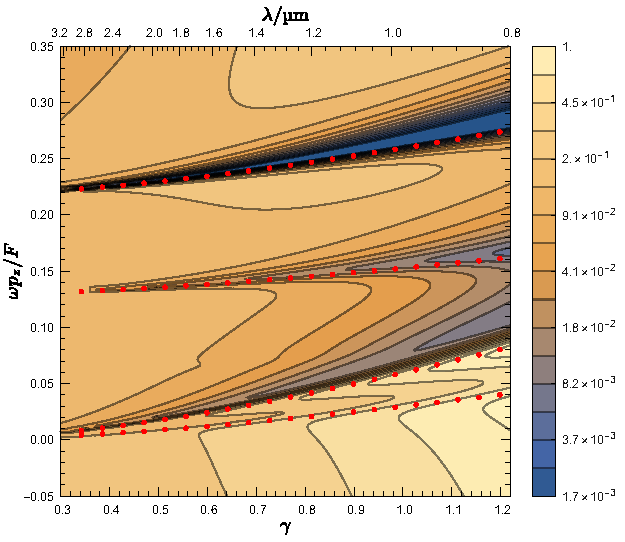
\includegraphics[scale=1]{6-LES/Figures/figure6-2C.pdf}
  \caption[
  Scaling of the ARM spectrum for 
  ]{
  Variation of the on-axis ionization amplitude $|a(\vbp)|^2$, in an arbitrary logarithmic scale, as a function of the wavelength and the corresponding Keldysh parameter~$\gamma$. The sudden drops in amplitude of \reffig{f6-po-pp-spectrum} shift along the momentum axis with a scaling that closely matches the classical soft-recollision trajectories, shown as red dots. Here the transverse momentum $\pp$ has been chosen so that the transverse coordinate of the classical trajectory has a small but positive value, $x = 1.07\tfrac{1}{\kappa}$, at the first soft recollision at $\omega t\approx 2\pi$, to avoid the hard singularity of the Coulomb kernel. 
  Here we take $F=\SI{\figuresixtwoCfield}{\au}$ $\kappa=\SI{\figuresixtwoCkappa}{\au}$, scaling $\gamma$ as a function of $\omega$ only.
  }
\label{f6-spectrum-scaling}
\end{figure}

In addition to the scaling dynamics, if the odd-$n$ do get lifted from consistent-with-zero by experiments with enough resolution, there is also a specific signature in the ratio of the momenta of the different structures within each series, which is relatively universal, coming from the fact that each series scales with $n$ as $1/(n+1)$, but with even $n$ for one and odd $n$ for the other. Thus, the momentum ratios between successive peaks of the LES series are expected to go down with $n$ as $3/5,5/7,7/9,\ldots$~\cite{Rost_PRL, Rost_JPhysB}, whereas the odd-$n$ series should scale down as $1/2,2/3,3/4,\ldots$. The way things stand, however, it will be hard enough to lift even the first peak out of the experimental zero of energy.





Coming back to the ARM results, the near-zero energy peaks shown in \reffig{f6-po-pp-spectrum}, along with similar peaks associated with the LES regime, scale exactly as they need to, which we show in \reffig{f6-spectrum-scaling}: the sharp changes in the spectrum, caused by the soft recollisions' topological transition, closely track the classical soft recollision scaling of \reffig{f6-soft-recollision-scaling}, underscoring the fundamental link between the two.


In this connection, it is worth remarking here that the soft recollisions, a crucial concept for our (seemingly abstract) branch-cut navigation algorithm of chapter~\ref{chap:quantum-orbits}, are brought directly to experimental life in the form of the Low-Energy Structures. The navigation algorithm is completely dependent on the resolution of the soft recollisions, but more importantly it requires the solution of both the even-$n$ and the odd-$n$ families to allow for fully functional ARM spectra in linear fields. 

Thus, it is the abstract branch-cut navigation that makes the discovery of the odd-$n$ soft recollision series inescapable (in contrast, for example to other approaches, where the odd-$n$ series is still present, but it is by nature much easier to miss); our account of the NZES therefore underscores the importance of the branch-cut navigation formalism. Other recent applications, in a higher-energy scenario, also underscore this~\cite{keil_branch-cuts_2016}.



Finally, it is also important to point out that, irrespective of the precise mechanism which translates the soft-recolliding trajectories into peaks in the photoelectron spectrum -- which can be the ARM method of tracking imaginary phases over laser-driven trajectories, but also the CCSFA method with semiclassical calculations on top of full trajectories, the ISFA interpretation in terms of single Born scattering terms, or the Monte Carlo focusing mechanism -- it is quite clear that the even-$n$ trajectories shown in \reffig{f6-trajectories-at-transitions} translate into photoelectron energy peaks, and the same should apply for the odd-$n$ trajectories, which are dynamically very similar. This can be seen, for example, in \reffig{f6-kelvich-dynamical-map}, where the first odd-$n$ recollision causes a caustic similar to the one behind the standard LES, but at NZES energies, but a closer investigation is required, on all of the mechanisms, to establish the exact nature of the connection and the contribution of this mechanism to the NZES.














%\subsection{Outlook}
%
%
%
%
%\cite{streaking_soft_recollisions}
























